\chapter{线性方程组与二次型}

% SOURCE_PDF_PAGE 101

\hypertarget{source-p101}{}
\phantomsection\addcontentsline{toc}{section}{2.1 竞赛要点与难点}
\phantomsection\addcontentsline{toc}{section}{2.2 范例解析与精讲}
在第1 章，我们重点讨论了行列式、矩阵以及矩阵特征值、特征向量等内容.本章主
要讨论向量、线性方程组和二次型.
\section*{2.1 竞赛要点与难点}
\par\noindent (1) Gauss (高斯)消元法、线性方程组的初等变换、线性方程组的一般解.
\par\noindent (2) 向量与向量组.{\symbolfont ①}向量: $n$维向量的运算，向量空间的定义及性质;{\symbolfont ①}向量组:向
量组的定义与等价，向量组的线性组合、线性相关与线性无关、向量组的极大无关组、向
量组的秩.
\par\noindent (3) 向量空间(线'性空间):线性空间的定义与简单性质、维数、基与坐标、基变换与
坐标变换、线性子空间.
\par\noindent (4) 子空间的交与和、维数公式、子空间的直和.
\par\noindent (5) 线性变换的值域与核、不变子空间、线性空间的分解与同构.
\par\noindent (6) 线性方程组求解:齐次线性方程组的基础解系、解空间及其维数;线性方程组有
解判别定理、线性方程组解唯一判别定理、线性方程组求解方法、线性方程组解的结构等.
\par\noindent (7) 双线性函数、对偶空间.
\par\noindent (8) 二次型: 二次型及其矩阵表示、矩阵的合同;二次型的标准形、化二次型为标准
形的配方法、合同变换法等;复数域和实数域上二次型的规范形的唯一性、惯性定理等.
\par\noindent (9) 正定、半正定、负定、半负定二次型及正定、半正定矩阵，负定、半负定矩阵的
性质与判定.
\par\noindent (10) 内积定义与基本性质:内积和欧氏空间、向量的长度、夹角与正交、度量矩阵，
标准正交基、正交矩阵、Schmidt (施密特)正交化方法等.
\par\noindent (11) 欧氏空间的同构，正交变换、子空间的正交补，对称变换、实对称矩阵的标准形.
\par\noindent (12) 主轴定理、用正交变换化实二次型或实对称矩阵为标准形.
\par\noindent (13) 国空间.
范例解析与精讲问
团组型-旬萤础性和英份以4 乱的租来似创刊
一般地，向量组的秩的计算可以通过定义而得到. 实际中，由于向量组的秩等于其作
为列(或行)向量组构成的矩阵的秩，因此，它可通过将该向量组构成的矩阵化为行阶梯


% SOURCE_PDF_PAGE 102

\hypertarget{source-p102}{}
形，计算该行阶梯形的非霉行的个数即可.
\sourceblock{450.00}{images-full/p102-d000.png}
\par\noindent (1) 向量组\allowbreak{}\raisebox{-2.16pt}{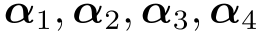
\includegraphics[width=74.01pt]{images-full/p102-i000.png}}\allowbreak{} 是否线性相关?
\par\noindent (2) 向量\allowbreak{}\raisebox{-2.76pt}{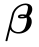
\includegraphics[width=10.73pt]{images-full/p102-i001.png}}\allowbreak{} 能否由向量组\allowbreak{}\raisebox{-2.16pt}{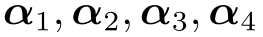
\includegraphics[width=74.01pt]{images-full/p102-i002.png}}\allowbreak{}线性表出?若能表示，写出表示式.
解(1) 将\allowbreak{}\raisebox{-2.04pt}{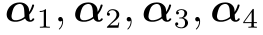
\includegraphics[width=74.01pt]{images-full/p102-i003.png}}\allowbreak{}拼成矩阵
\sourceblock{122.60}{images-full/p102-d001.png}
将其化为行阶梯形，即
\sourceblock{270.63}{images-full/p102-d002.png}
故\allowbreak{}\raisebox{-2.04pt}{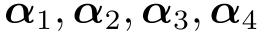
\includegraphics[width=74.01pt]{images-full/p102-i004.png}}\allowbreak{}线性无关.
\par\noindent (2) 将$A$ 扩展为
\sourceblock{189.84}{images-full/p102-d003.png}
将其化为行最简形，即
\sourceblock{450.00}{images-full/p102-d004.png}
\sourceblock{450.00}{images-full/p102-d005.png}
的线性相关性.


% SOURCE_PDF_PAGE 103

\hypertarget{source-p103}{}
解第一种情形:当\allowbreak{}\raisebox{-2.04pt}{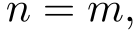
\includegraphics[width=38.91pt]{images-full/p103-i000.png}}\allowbreak{}且\allowbreak{}\raisebox{-2.52pt}{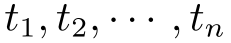
\includegraphics[width=64.97pt]{images-full/p103-i001.png}}\allowbreak{} 互异时，由Vandermonde 行列式知，\allowbreak{}\raisebox{-2.16pt}{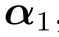
\includegraphics[width=16.38pt]{images-full/p103-i002.png}}\allowbreak{}
\allowbreak{}\raisebox{-2.16pt}{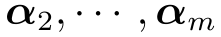
\includegraphics[width=62.15pt]{images-full/p103-i003.png}}\allowbreak{} 线性无关.
第二种情形:当\allowbreak{}\raisebox{-2.04pt}{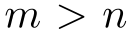
\includegraphics[width=37.85pt]{images-full/p103-i004.png}}\allowbreak{} 时，此时向量组中的向量个数大于这些向量所在的向量空间
的维数，因此必线性相关.
第三种情形: 当\allowbreak{}\raisebox{-1.92pt}{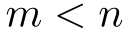
\includegraphics[width=36.16pt]{images-full/p103-i005.png}}\allowbreak{} 时，考察矩阵
\sourceblock{266.68}{images-full/p103-d000.png}
若\allowbreak{}\raisebox{-2.52pt}{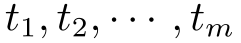
\includegraphics[width=67.80pt]{images-full/p103-i006.png}}\allowbreak{} 各不相同，则\allowbreak{}\raisebox{-3.00pt}{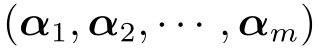
\includegraphics[width=89.83pt]{images-full/p103-i007.png}}\allowbreak{} 有$m$ 阶子式不为\allowbreak{}\raisebox{-2.64pt}{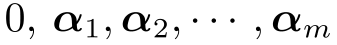
\includegraphics[width=94.92pt]{images-full/p103-i009.png}}\allowbreak{}
线性无关.若虹\allowbreak{}\raisebox{-2.52pt}{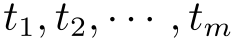
\includegraphics[width=67.23pt]{images-full/p103-i010.png}}\allowbreak{} 有两个相同，则(\allowbreak{}\raisebox{-3.00pt}{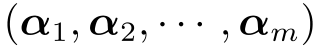
\includegraphics[width=90.40pt]{images-full/p103-i011.png}}\allowbreak{} 至少有两列相同，从而
\allowbreak{}\raisebox{-2.04pt}{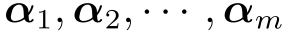
\includegraphics[width=81.36pt]{images-full/p103-i012.png}}\allowbreak{} 线性相关.
\sourceblock{314.14}{images-full/p103-d001.png}
\par\medskip\noindent\textbf{【例2.2.41给定实数酌\allowbreak{}\raisebox{-2.04pt}{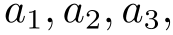
\includegraphics[width=48.63pt]{images-full/p104-i000.png}}\allowbreak{}，利用关系式}
\sourceblock{214.13}{images-full/p104-d000.png}
得到数列\allowbreak{}\raisebox{-3.24pt}{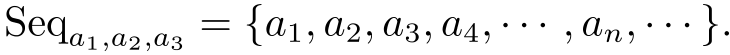
\includegraphics[width=205.88pt]{images-full/p104-i001.png}}\allowbreak{}.令\allowbreak{}\raisebox{-3.24pt}{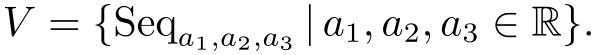
\includegraphics[width=167.18pt]{images-full/p104-i002.png}}\allowbreak{}
\par\noindent (1) 证明:$V$ 关于数列的通常加法以及实数对数列的通常乘法构成一个实向量空间，
其维数为3.
\par\noindent (2) 试求出数列\allowbreak{}\raisebox{-3.12pt}{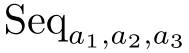
\includegraphics[width=53.11pt]{images-full/p104-i004.png}}\allowbreak{} 的通项式\allowbreak{}\raisebox{-2.04pt}{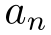
\includegraphics[width=14.12pt]{images-full/p104-i005.png}}\allowbreak{} 的表达式
\par\noindent (1) 证明直接验证可知，$V$ 关于题目所给的向量加法与数乘满足向量壁间定义的8
条公理，从而$V$ 构成一个实向量空间.
\sourceblock{382.50}{images-full/p104-d001.png}
\sourceblock{146.33}{images-full/p104-d002.png}
可知，\allowbreak{}\raisebox{-3.24pt}{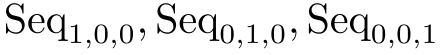
\includegraphics[width=124.86pt]{images-full/p104-i008.png}}\allowbreak{}为线性无关向量组，且\allowbreak{}\raisebox{-3.24pt}{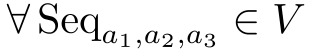
\includegraphics[width=87.57pt]{images-full/p104-i009.png}}\allowbreak{} 的前三项为吨\allowbreak{}\raisebox{-2.16pt}{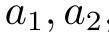
\includegraphics[width=30.62pt]{images-full/p104-i010.png}}\allowbreak{}，
\allowbreak{}\raisebox{-2.04pt}{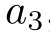
\includegraphics[width=13.94pt]{images-full/p104-i011.png}}\allowbreak{}记
\sourceblock{111.30}{images-full/p104-d003.png}
于是
\sourceblock{107.35}{images-full/p104-d004.png}
进而\allowbreak{}\raisebox{-2.76pt}{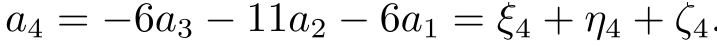
\includegraphics[width=202.14pt]{images-full/p104-i012.png}}\allowbreak{} 一般地，应用数学归纳法可得
\sourceblock{97.74}{images-full/p104-d005.png}
\sourceblock{392.67}{images-full/p104-d006.png}
\par\noindent (2) 由递推关系式可知
\sourceblock{214.70}{images-full/p104-d007.png}


% SOURCE_PDF_PAGE 105

\hypertarget{source-p105}{}
进而
\sourceblock{305.10}{images-full/p105-d000.png}
\sourceblock{429.40}{images-full/p105-d001.png}
\sourceblock{301.14}{images-full/p105-d002.png}


% SOURCE_PDF_PAGE 106

\hypertarget{source-p106}{}
\sourceblock{409.62}{images-full/p106-d000.png}
\allowbreak{}\raisebox{-2.88pt}{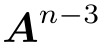
\includegraphics[width=29.38pt]{images-full/p106-i000.png}}\allowbreak{} 的第一行为
\sourceblock{450.00}{images-full/p106-d001.png}
故\allowbreak{}\raisebox{-3.24pt}{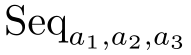
\includegraphics[width=53.67pt]{images-full/p106-i001.png}}\allowbreak{} 的第\allowbreak{}\raisebox{-1.68pt}{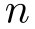
\includegraphics[width=9.60pt]{images-full/p106-i002.png}}\allowbreak{} 项\allowbreak{}\raisebox{-2.04pt}{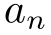
\includegraphics[width=14.12pt]{images-full/p106-i003.png}}\allowbreak{} 的表达式为
\sourceblock{347.47}{images-full/p106-d002.png}
\par\medskip\noindent\textbf{【例2.2.7】设\allowbreak{}\raisebox{-2.16pt}{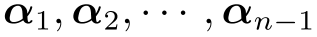
\includegraphics[width=89.27pt]{images-full/p108-i002.png}}\allowbreak{} 为]\allowbreak{}\raisebox{-2.28pt}{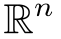
\includegraphics[width=16.95pt]{images-full/p108-i003.png}}\allowbreak{} 中线性无关的向量组，且\allowbreak{}\raisebox{-3.00pt}{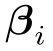
\includegraphics[width=14.69pt]{images-full/p108-i004.png}}\allowbreak{}与\allowbreak{}\raisebox{-2.16pt}{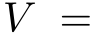
\includegraphics[width=27.12pt]{images-full/p108-i005.png}}\allowbreak{}}
\allowbreak{}\raisebox{-3.00pt}{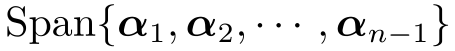
\includegraphics[width=128.25pt]{images-full/p108-i006.png}}\allowbreak{} 垂直，\allowbreak{}\raisebox{-3.00pt}{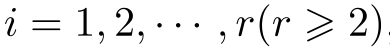
\includegraphics[width=109.85pt]{images-full/p108-i007.png}}\allowbreak{}，证明:\allowbreak{}\raisebox{-2.88pt}{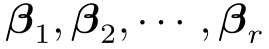
\includegraphics[width=75.71pt]{images-full/p108-i008.png}}\allowbreak{}必线性相关
\par\noindent\textbf{证明}\ 由\allowbreak{}\raisebox{-3.00pt}{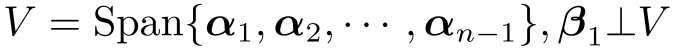
\includegraphics[width=190.97pt]{images-full/p108-i009.png}}\allowbreak{} 知，若
\sourceblock{226.56}{images-full/p108-d001.png}
两边与\allowbreak{}\raisebox{-3.00pt}{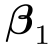
\includegraphics[width=15.25pt]{images-full/p108-i010.png}}\allowbreak{}作内积
\sourceblock{303.40}{images-full/p108-d002.png}
即
\sourceblock{280.24}{images-full/p108-d003.png}
进而得\allowbreak{}\raisebox{-3.00pt}{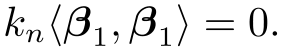
\includegraphics[width=79.38pt]{images-full/p108-i011.png}}\allowbreak{} 当\allowbreak{}\raisebox{-2.88pt}{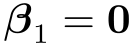
\includegraphics[width=38.42pt]{images-full/p108-i012.png}}\allowbreak{} 时，显然\allowbreak{}\raisebox{-2.88pt}{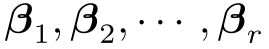
\includegraphics[width=75.71pt]{images-full/p108-i013.png}}\allowbreak{} 线性相关，如所需.
\sourceblock{431.66}{images-full/p108-d004.png}
\allowbreak{}\raisebox{-2.04pt}{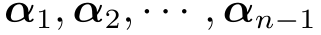
\includegraphics[width=90.40pt]{images-full/p108-i014.png}}\allowbreak{} 是线性无关向量组得\allowbreak{}\raisebox{-2.64pt}{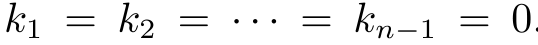
\includegraphics[width=151.75pt]{images-full/p108-i015.png}}\allowbreak{} 因此，此时有\allowbreak{}\raisebox{-3.00pt}{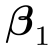
\includegraphics[width=15.25pt]{images-full/p108-i016.png}}\allowbreak{}
与\allowbreak{}\raisebox{-2.16pt}{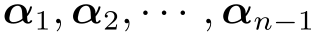
\includegraphics[width=89.27pt]{images-full/p108-i017.png}}\allowbreak{}构成一个线性无关向量组，其向量个数为$n$，从而它能作为]\allowbreak{}\raisebox{-2.28pt}{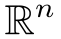
\includegraphics[width=16.95pt]{images-full/p108-i019.png}}\allowbreak{} 的一
组基.此时\allowbreak{}\raisebox{-2.88pt}{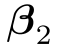
\includegraphics[width=15.82pt]{images-full/p108-i020.png}}\allowbreak{}可由\allowbreak{}\raisebox{-2.88pt}{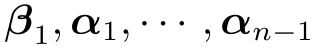
\includegraphics[width=89.27pt]{images-full/p108-i021.png}}\allowbreak{}线性表出
\sourceblock{190.40}{images-full/p108-d005.png}
若β2 =0，则显见，矶，肉，…，β俨线性相关，获证
\sourceblock{450.00}{images-full/p108-d006.png}
\allowbreak{}\raisebox{-2.88pt}{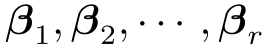
\includegraphics[width=75.71pt]{images-full/p108-i022.png}}\allowbreak{} 线性相关.口
\par\medskip\noindent\textbf{【例2.2.8 】证明:对任意正交矩阵$A$，必存在正交矩阵$Q$，使得}


% SOURCE_PDF_PAGE 109

\hypertarget{source-p109}{}
\sourceblock{403.97}{images-full/p109-d000.png}
\par\noindent\textbf{证明}\ 我们考察\allowbreak{}\raisebox{-1.68pt}{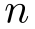
\includegraphics[width=9.60pt]{images-full/p109-i000.png}}\allowbreak{}维实内积空间$V$ 相应于$A$ 的正交变换\allowbreak{}\raisebox{-2.28pt}{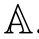
\includegraphics[width=10.61pt]{images-full/p109-i003.png}}\allowbreak{} 将$V$ 变化为西空间
\allowbreak{}\raisebox{-3.00pt}{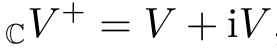
\includegraphics[width=78.16pt]{images-full/p109-i005.png}}\allowbreak{}，同时也将$A$ 复化为\allowbreak{}\raisebox{-3.00pt}{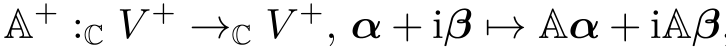
\includegraphics[width=204.87pt]{images-full/p109-i007.png}}\allowbreak{}，则有\allowbreak{}\raisebox{-2.52pt}{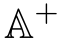
\includegraphics[width=18.08pt]{images-full/p109-i008.png}}\allowbreak{} 仍
为西变换.稍作推导即知，\allowbreak{}\raisebox{-2.64pt}{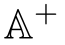
\includegraphics[width=18.08pt]{images-full/p109-i009.png}}\allowbreak{}还具有以下性质:
\par\noindent (1) \allowbreak{}\raisebox{-2.52pt}{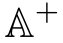
\includegraphics[width=17.51pt]{images-full/p109-i010.png}}\allowbreak{} 的非实特征值必共辄成对出现.若用\allowbreak{}\raisebox{-3.12pt}{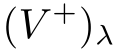
\includegraphics[width=33.33pt]{images-full/p109-i011.png}}\allowbreak{} 表示\allowbreak{}\raisebox{-2.52pt}{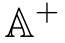
\includegraphics[width=18.08pt]{images-full/p109-i012.png}}\allowbreak{}关于\allowbreak{}\raisebox{-2.28pt}{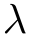
\includegraphics[width=9.04pt]{images-full/p109-i013.png}}\allowbreak{} 的特征于空间，
则映射\allowbreak{}\raisebox{-3.36pt}{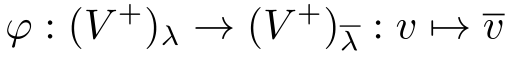
\includegraphics[width=144.07pt]{images-full/p109-i014.png}}\allowbreak{}为一一对应.
\par\noindent (2) \allowbreak{}\raisebox{-2.52pt}{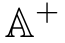
\includegraphics[width=18.08pt]{images-full/p109-i015.png}}\allowbreak{} 的西性保证了\allowbreak{}\raisebox{-2.52pt}{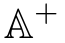
\includegraphics[width=18.08pt]{images-full/p109-i016.png}}\allowbreak{} 的两个互异特征子空间相互垂直.进一步，当特征值\allowbreak{}\raisebox{-2.28pt}{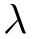
\includegraphics[width=9.04pt]{images-full/p109-i017.png}}\allowbreak{} 不
为实数时，若\allowbreak{}\raisebox{-3.24pt}{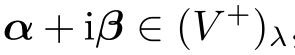
\includegraphics[width=83.21pt]{images-full/p109-i018.png}}\allowbreak{}，则由\allowbreak{}\raisebox{-3.36pt}{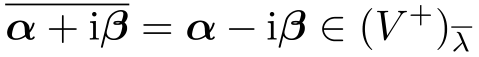
\includegraphics[width=135.03pt]{images-full/p109-i019.png}}\allowbreak{} 以及\allowbreak{}\raisebox{-3.24pt}{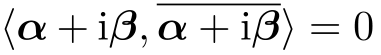
\includegraphics[width=107.35pt]{images-full/p109-i020.png}}\allowbreak{}
得
\sourceblock{158.20}{images-full/p109-d001.png}
因此，若\allowbreak{}\raisebox{-5.00pt}{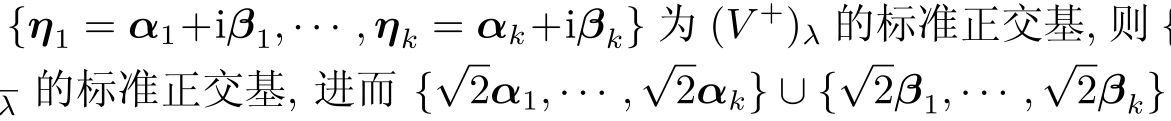
\includegraphics[width=330.43pt]{images-full/p109-i021.png}}\allowbreak{}\allowbreak{}\raisebox{-5.00pt}{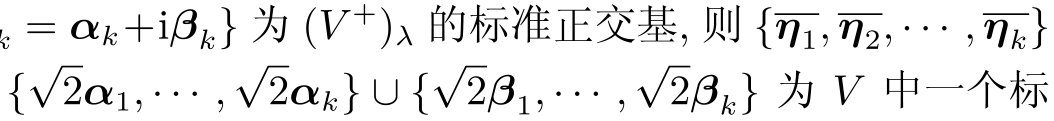
\includegraphics[width=297.61pt]{images-full/p109-i023.png}}\allowbreak{}
为\allowbreak{}\raisebox{-3.24pt}{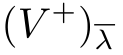
\includegraphics[width=34.46pt]{images-full/p109-i024.png}}\allowbreak{}
准正交基.
\par\noindent (3) \allowbreak{}\raisebox{-2.52pt}{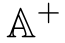
\includegraphics[width=18.08pt]{images-full/p109-i025.png}}\allowbreak{} 的特征值均坐落在单位圆周上. \allowbreak{}\raisebox{-2.52pt}{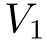
\includegraphics[width=12.99pt]{images-full/p109-i026.png}}\allowbreak{} 表示$A$ 关于\allowbreak{}\raisebox{-2.16pt}{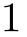
\includegraphics[width=7.34pt]{images-full/p109-i028.png}}\allowbreak{} 的特征子空间\allowbreak{}\raisebox{-2.52pt}{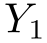
\includegraphics[width=12.99pt]{images-full/p109-i029.png}}\allowbreak{}且为\allowbreak{}\raisebox{-2.52pt}{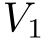
\includegraphics[width=12.43pt]{images-full/p109-i030.png}}\allowbreak{}的
一组标准正交基; \allowbreak{}\raisebox{-2.64pt}{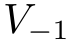
\includegraphics[width=20.34pt]{images-full/p109-i031.png}}\allowbreak{}表示$A$ 关于\allowbreak{}\raisebox{-2.16pt}{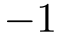
\includegraphics[width=16.95pt]{images-full/p109-i033.png}}\allowbreak{}的$V$ 的特征子壁间，\allowbreak{}\raisebox{-2.64pt}{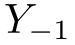
\includegraphics[width=20.90pt]{images-full/p109-i035.png}}\allowbreak{}为\allowbreak{}\raisebox{-2.64pt}{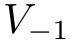
\includegraphics[width=20.34pt]{images-full/p109-i036.png}}\allowbreak{} 的一组标准正交
基，则由
\sourceblock{129.38}{images-full/p109-d002.png}
得\allowbreak{}\raisebox{-2.76pt}{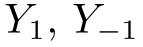
\includegraphics[width=40.11pt]{images-full/p109-i037.png}}\allowbreak{}也分别是\allowbreak{}\raisebox{-3.12pt}{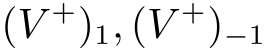
\includegraphics[width=75.71pt]{images-full/p109-i038.png}}\allowbreak{} 的标准正交基
综上所述有


% SOURCE_PDF_PAGE 110

\hypertarget{source-p110}{}
\sourceblock{415.27}{images-full/p110-d000.png}
则由\allowbreak{}\raisebox{-3.00pt}{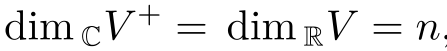
\includegraphics[width=126.00pt]{images-full/p110-i000.png}}\allowbreak{}，可得
\sourceblock{356.51}{images-full/p110-d001.png}
构成\allowbreak{}\raisebox{-2.64pt}{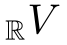
\includegraphics[width=18.64pt]{images-full/p110-i001.png}}\allowbreak{} 的一组标准正交基，$A$ 在此基下的矩阵为
\sourceblock{347.47}{images-full/p110-d002.png}
口
团组型四川钱性方程组在钱性方程组伪解错精
\sourceblock{432.79}{images-full/p110-d003.png}
空间，非齐次线性方程组的解是一个超平面(即为一个特解加上其对应齐次线性方程组的
解空间).而针对含参线性方程组的解的讨论，其方法一般可归纳为: 首先对线性方程组作
初等变换，将其化为阶梯形方程组;其次根据参数的不同取值，讨论方程组是无解、有唯
一解还是有无穷多解.
\par\medskip\noindent\textbf{【例2.2.11 】设3 阶实对称矩阵的三个特征值为一1.1.1. A 的与特征值-1 相应}
\sourceblock{204.53}{images-full/p112-d005.png}


% SOURCE_PDF_PAGE 113

\hypertarget{source-p113}{}
i
解用\allowbreak{}\raisebox{-2.64pt}{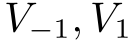
\includegraphics[width=37.29pt]{images-full/p113-i000.png}}\allowbreak{}分别表示$A$ 关于\allowbreak{}\raisebox{-2.16pt}{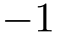
\includegraphics[width=16.38pt]{images-full/p113-i002.png}}\allowbreak{}阳的特征子空间则有\allowbreak{}\raisebox{-2.76pt}{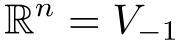
\includegraphics[width=50.98pt]{images-full/p113-i003.png}}\allowbreak{}EB\allowbreak{}\raisebox{-2.64pt}{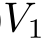
\includegraphics[width=12.99pt]{images-full/p113-i004.png}}\allowbreak{}，因此
有\allowbreak{}\raisebox{-3.24pt}{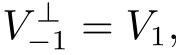
\includegraphics[width=49.55pt]{images-full/p113-i005.png}}\allowbreak{}，亦即
\sourceblock{428.83}{images-full/p113-d000.png}
$n$ 阶矩阵$A$ 可相似对角化的充要条件是它有\allowbreak{}\raisebox{-1.56pt}{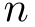
\includegraphics[width=9.60pt]{images-full/p113-i008.png}}\allowbreak{}个线性无关的特征向量，它又等价于
$A$ 的每个特征值\allowbreak{}\raisebox{-2.28pt}{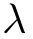
\includegraphics[width=9.04pt]{images-full/p113-i010.png}}\allowbreak{} 的几何重数等于其代数重数.复数域上，可对角化矩阵即为正规矩阵
(即满足\allowbreak{}\raisebox{-2.40pt}{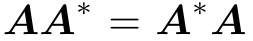
\includegraphics[width=71.19pt]{images-full/p113-i011.png}}\allowbreak{} 的方阵\allowbreak{}\raisebox{-2.40pt}{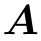
\includegraphics[width=11.40pt]{images-full/p113-i012.png}}\allowbreak{}. 特别地，实对称矩阵、自共辄矩阵均是可对角化矩阵.
当然，正交矩阵与国矩阵也都是可对角化矩阵(将它们统一看成复数域上的矩阵情况下) .
\sourceblock{433.35}{images-full/p113-d001.png}
随矩阵
\sourceblock{263.85}{images-full/p113-d002.png}
若\allowbreak{}\raisebox{-3.00pt}{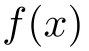
\includegraphics[width=24.86pt]{images-full/p113-i013.png}}\allowbreak{} 在$C$ 上有$n$个不同的根，试求一可逆矩阵$P$，使得
\sourceblock{160.46}{images-full/p113-d003.png}


% SOURCE_PDF_PAGE 114

\hypertarget{source-p114}{}
\sourceblock{424.31}{images-full/p114-d000.png}
\sourceblock{208.48}{images-full/p114-d001.png}
\sourceblock{422.05}{images-full/p114-d002.png}
注意到\allowbreak{}\raisebox{-2.64pt}{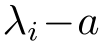
\includegraphics[width=29.94pt]{images-full/p114-i000.png}}\allowbreak{}与\allowbreak{}\raisebox{-3.24pt}{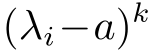
\includegraphics[width=43.50pt]{images-full/p114-i001.png}}\allowbreak{} 同时为\allowbreak{}\raisebox{-2.28pt}{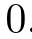
\includegraphics[width=8.93pt]{images-full/p114-i002.png}}\allowbreak{} 因此\allowbreak{}\raisebox{-3.00pt}{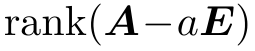
\includegraphics[width=71.75pt]{images-full/p114-i003.png}}\allowbreak{} 等于\allowbreak{}\raisebox{-2.76pt}{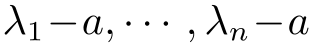
\includegraphics[width=89.27pt]{images-full/p114-i004.png}}\allowbreak{} 中非零
元的个数\allowbreak{}\raisebox{-2.04pt}{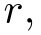
\includegraphics[width=11.30pt]{images-full/p114-i005.png}}\allowbreak{}当然也就是\allowbreak{}\raisebox{-3.36pt}{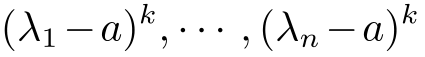
\includegraphics[width=119.78pt]{images-full/p114-i006.png}}\allowbreak{} 中非零元的个数.故有\allowbreak{}\raisebox{-3.36pt}{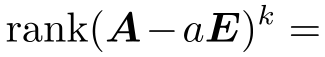
\includegraphics[width=91.53pt]{images-full/p114-i007.png}}\allowbreak{}
\allowbreak{}\raisebox{-3.00pt}{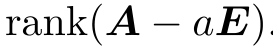
\includegraphics[width=77.01pt]{images-full/p114-i008.png}}\allowbreak{}口
\par\medskip\noindent\textbf{【例2.2.14 】设$A$ 是\allowbreak{}\raisebox{-1.80pt}{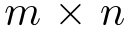
\includegraphics[width=37.29pt]{images-full/p114-i010.png}}\allowbreak{} 复矩阵，证明:\allowbreak{}\raisebox{-2.40pt}{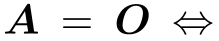
\includegraphics[width=61.58pt]{images-full/p114-i011.png}}\allowbreak{}存在自然数$k$，使得}
\allowbreak{}\raisebox{-3.24pt}{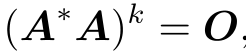
\includegraphics[width=69.28pt]{images-full/p114-i013.png}}\allowbreak{}，其中\allowbreak{}\raisebox{-2.40pt}{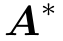
\includegraphics[width=17.51pt]{images-full/p114-i014.png}}\allowbreak{}表示$A$ 的共辄转置.


% SOURCE_PDF_PAGE 115

\hypertarget{source-p115}{}
\par\noindent\textbf{证明}\ 充分性易知，\allowbreak{}\raisebox{-2.40pt}{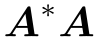
\includegraphics[width=28.25pt]{images-full/p115-i000.png}}\allowbreak{}是自共辄矩阵，因此官可国对角化.亦即存在西矩阵$U$使得
\sourceblock{346.91}{images-full/p115-d000.png}
故有\allowbreak{}\raisebox{-2.52pt}{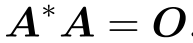
\includegraphics[width=54.32pt]{images-full/p115-i002.png}}\allowbreak{} 注意到，\allowbreak{}\raisebox{-3.00pt}{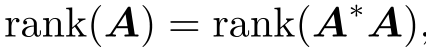
\includegraphics[width=120.10pt]{images-full/p115-i003.png}}\allowbreak{}，因此\allowbreak{}\raisebox{-2.40pt}{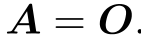
\includegraphics[width=39.49pt]{images-full/p115-i004.png}}\allowbreak{}
必要性是显然的.口
【点评】在竞赛中，关于实对称阵的对角化问题的考察重点，往往是考察如何将一
实对称阵实现其正交相似对角化的问题，困为它实际上是给出了将一个二次型化为标准
形的过程(坐标变换与标准形同时被给出).
\par\medskip\noindent\textbf{【例2.2.17 】设2024 阶实对称阵$A$ 的秩为1010，且满足\allowbreak{}\raisebox{-2.76pt}{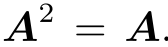
\includegraphics[width=47.37pt]{images-full/p117-i006.png}}\allowbreak{} 求二次型}
\allowbreak{}\raisebox{-2.76pt}{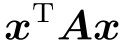
\includegraphics[width=35.50pt]{images-full/p117-i007.png}}\allowbreak{}z:的规范形，并计算行列式\allowbreak{}\raisebox{-3.48pt}{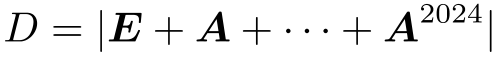
\includegraphics[width=140.68pt]{images-full/p117-i008.png}}\allowbreak{} 的值.
解\allowbreak{}\raisebox{-2.76pt}{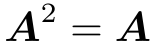
\includegraphics[width=44.07pt]{images-full/p117-i009.png}}\allowbreak{}表明$A$ 的特征值为:\allowbreak{}\raisebox{-2.64pt}{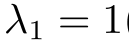
\includegraphics[width=36.15pt]{images-full/p117-i011.png}}\allowbreak{}(其重数为1010) ，\allowbreak{}\raisebox{-2.64pt}{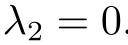
\includegraphics[width=35.81pt]{images-full/p117-i012.png}}\allowbreak{}.
故
\sourceblock{222.04}{images-full/p117-d003.png}
\sourceblock{240.12}{images-full/p117-d004.png}
\par\medskip\noindent\textbf{【例2.2.18 】求函数}
\sourceblock{234.47}{images-full/p117-d005.png}
的最大值与最小值，并找出最大值点和最小值点.
解令
\sourceblock{232.21}{images-full/p117-d006.png}
此为三元实二次型.取正交变换
\sourceblock{115.26}{images-full/p117-d007.png}


% SOURCE_PDF_PAGE 118

\hypertarget{source-p118}{}
\sourceblock{383.63}{images-full/p118-d000.png}
\sourceblock{102.26}{images-full/p118-d001.png}
\sourceblock{450.00}{images-full/p118-d002.png}
$k$ 为任意非军实数.
类似地可得:$f$ 的最小值为\allowbreak{}\raisebox{-2.64pt}{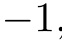
\includegraphics[width=17.20pt]{images-full/p118-i002.png}}\allowbreak{}，其最小值点为
\sourceblock{259.90}{images-full/p118-d003.png}
\sourceblock{450.00}{images-full/p118-d004.png}
\par\medskip\noindent\textbf{【例2.2.19 】己知三元实二次型\allowbreak{}\raisebox{-3.24pt}{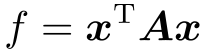
\includegraphics[width=58.19pt]{images-full/p118-i003.png}}\allowbreak{} 经正交变换后所得的标准形为}
\sourceblock{74.01}{images-full/p118-d005.png}


% SOURCE_PDF_PAGE 119

\hypertarget{source-p119}{}
\sourceblock{320.92}{images-full/p119-d000.png}
\sourceblock{450.00}{images-full/p119-d001.png}
解根据题设知，$A$ 的特征值为\allowbreak{}\raisebox{-2.76pt}{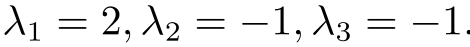
\includegraphics[width=132.55pt]{images-full/p119-i001.png}}\allowbreak{}.从而\allowbreak{}\raisebox{-3.00pt}{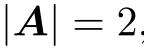
\includegraphics[width=40.47pt]{images-full/p119-i002.png}}\allowbreak{}，进而
\sourceblock{278.54}{images-full/p119-d002.png}
矩阵$B$ 满足
\sourceblock{347.47}{images-full/p119-d003.png}
由此得\allowbreak{}\raisebox{-3.24pt}{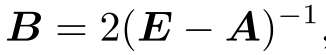
\includegraphics[width=91.99pt]{images-full/p119-i004.png}}\allowbreak{}，故$B$ 的特征值为\allowbreak{}\raisebox{-2.64pt}{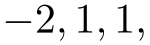
\includegraphics[width=41.91pt]{images-full/p119-i006.png}}\allowbreak{}，且\allowbreak{}\raisebox{-2.28pt}{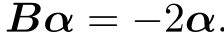
\includegraphics[width=63.10pt]{images-full/p119-i007.png}}\allowbreak{}.
\sourceblock{450.00}{images-full/p119-d004.png}
\sourceblock{66.67}{images-full/p119-d005.png}
由此可得\allowbreak{}\raisebox{-2.64pt}{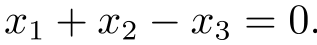
\includegraphics[width=89.31pt]{images-full/p119-i008.png}}\allowbreak{} 解得其基础解系为
\sourceblock{106.78}{images-full/p119-d006.png}


% SOURCE_PDF_PAGE 120

\hypertarget{source-p120}{}
\sourceblock{383.63}{images-full/p120-d000.png}
\par\medskip\noindent\textbf{【例2.2.20 】设\allowbreak{}\raisebox{-2.64pt}{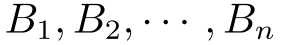
\includegraphics[width=79.10pt]{images-full/p120-i000.png}}\allowbreak{} 为实平面\allowbreak{}\raisebox{-2.64pt}{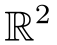
\includegraphics[width=15.82pt]{images-full/p120-i001.png}}\allowbreak{}上的$n$个半径不为\allowbreak{}\raisebox{-2.28pt}{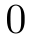
\includegraphics[width=9.04pt]{images-full/p120-i003.png}}\allowbreak{} 的圆.记\allowbreak{}\raisebox{-2.88pt}{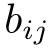
\includegraphics[width=14.69pt]{images-full/p120-i004.png}}\allowbreak{}为}
圆\allowbreak{}\raisebox{-2.76pt}{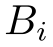
\includegraphics[width=14.69pt]{images-full/p120-i005.png}}\allowbreak{}与圆\allowbreak{}\raisebox{-3.00pt}{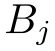
\includegraphics[width=15.25pt]{images-full/p120-i006.png}}\allowbreak{}的相交部分的面积. 令\allowbreak{}\raisebox{-3.12pt}{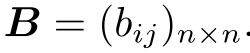
\includegraphics[width=70.30pt]{images-full/p120-i007.png}}\allowbreak{} 证明: \allowbreak{}\raisebox{-3.00pt}{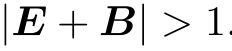
\includegraphics[width=65.27pt]{images-full/p120-i008.png}}\allowbreak{}.
\par\noindent\textbf{证明}\ 设\allowbreak{}\raisebox{-2.28pt}{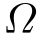
\includegraphics[width=11.86pt]{images-full/p120-i009.png}}\allowbreak{}为以\allowbreak{}\raisebox{-3.00pt}{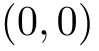
\includegraphics[width=27.68pt]{images-full/p120-i010.png}}\allowbreak{} 为中心，半径足够大使\allowbreak{}\raisebox{-2.76pt}{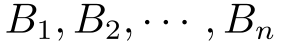
\includegraphics[width=79.10pt]{images-full/p120-i011.png}}\allowbreak{} 均包含在其内的圆
考察二次型
\sourceblock{314.70}{images-full/p120-d001.png}
\sourceblock{279.11}{images-full/p120-d002.png}
其中\allowbreak{}\raisebox{-2.16pt}{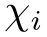
\includegraphics[width=12.99pt]{images-full/p120-i012.png}}\allowbreak{}表示\allowbreak{}\raisebox{-2.64pt}{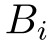
\includegraphics[width=14.69pt]{images-full/p120-i013.png}}\allowbreak{}在$Q$ 上的特征函数. 则有
\sourceblock{228.82}{images-full/p120-d003.png}
故$B$ 为半正定阵，且$B$ 的主对角元皆大于\allowbreak{}\raisebox{-2.16pt}{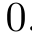
\includegraphics[width=8.70pt]{images-full/p120-i017.png}}\allowbreak{}
\sourceblock{450.00}{images-full/p120-d004.png}
口


% SOURCE_PDF_PAGE 121

\hypertarget{source-p121}{}
园时八堂制解在远躏
\par\medskip\noindent\textbf{【例2.2.24 】设f(功，g(x) 为实系数多项式，f 与g 互素.\allowbreak{}\raisebox{-1.56pt}{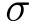
\includegraphics[width=10.17pt]{images-full/p123-i001.png}}\allowbreak{} 为\allowbreak{}\raisebox{-2.28pt}{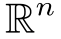
\includegraphics[width=16.95pt]{images-full/p123-i002.png}}\allowbreak{} 上的一个线性变}
\sourceblock{450.00}{images-full/p123-d001.png}
\sourceblock{67.80}{images-full/p123-d002.png}
则\allowbreak{}\raisebox{-3.00pt}{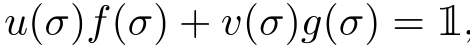
\includegraphics[width=132.45pt]{images-full/p123-i003.png}}\allowbreak{}，这里\allowbreak{}\raisebox{-2.28pt}{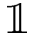
\includegraphics[width=9.60pt]{images-full/p123-i004.png}}\allowbreak{}表示恒等变换.进而\allowbreak{}\raisebox{-2.74pt}{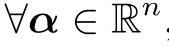
\includegraphics[width=47.45pt]{images-full/p123-i005.png}}\allowbreak{}，
\sourceblock{191.53}{images-full/p123-d003.png}
\sourceblock{393.80}{images-full/p123-d004.png}
\sourceblock{74.58}{images-full/p123-d005.png}
最后，若\allowbreak{}\raisebox{-2.76pt}{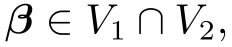
\includegraphics[width=65.23pt]{images-full/p123-i006.png}}\allowbreak{}，再次由等式\allowbreak{}\raisebox{-2.76pt}{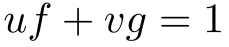
\includegraphics[width=64.41pt]{images-full/p123-i007.png}}\allowbreak{}知\allowbreak{}\raisebox{-2.76pt}{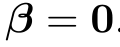
\includegraphics[width=33.72pt]{images-full/p123-i008.png}}\allowbreak{} 故有
\sourceblock{266.68}{images-full/p123-d006.png}
【点评】此例的结果表明:将\allowbreak{}\raisebox{-1.56pt}{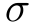
\includegraphics[width=9.60pt]{images-full/p123-i009.png}}\allowbreak{} 的特征多项式\allowbreak{}\raisebox{-3.00pt}{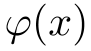
\includegraphics[width=25.42pt]{images-full/p123-i010.png}}\allowbreak{} 分解为\allowbreak{}\raisebox{-3.00pt}{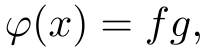
\includegraphics[width=56.04pt]{images-full/p123-i011.png}}\allowbreak{}，其中\allowbreak{}\raisebox{-2.88pt}{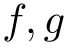
\includegraphics[width=19.77pt]{images-full/p123-i012.png}}\allowbreak{} 互
素.则有\allowbreak{}\raisebox{-2.76pt}{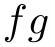
\includegraphics[width=15.25pt]{images-full/p123-i013.png}}\allowbreak{} 为\allowbreak{}\raisebox{-1.56pt}{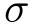
\includegraphics[width=10.17pt]{images-full/p123-i014.png}}\allowbreak{} 的零化多项式.若取\allowbreak{}\raisebox{-2.64pt}{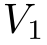
\includegraphics[width=12.99pt]{images-full/p123-i015.png}}\allowbreak{}的一组基并上\allowbreak{}\raisebox{-2.64pt}{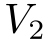
\includegraphics[width=13.56pt]{images-full/p123-i016.png}}\allowbreak{}的基，则\allowbreak{}\raisebox{-1.56pt}{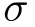
\includegraphics[width=9.60pt]{images-full/p123-i017.png}}\allowbreak{} 在此基下的表示阵
为分块对角矩阵.这正是建立线性变换(矩阵) Jordan 标准形的起始点.
\par\medskip\noindent\textbf{【例2.2.25 】设$V$ 是数域$K$ 上的$n$ 维线性空间，\allowbreak{}\raisebox{-1.68pt}{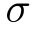
\includegraphics[width=10.17pt]{images-full/p123-i021.png}}\allowbreak{} 是$V$ 上的线性变换，且}
\sourceblock{225.43}{images-full/p123-d007.png}
设
\sourceblock{246.34}{images-full/p123-d008.png}
并满足f(σ)(α) 二o. 若f(x) 在K 上至少有两个互异的首一不可约因式，证明::3β ，γε
\sourceblock{409.62}{images-full/p123-d009.png}


% SOURCE_PDF_PAGE 124

\hypertarget{source-p124}{}
\phantomsection\addcontentsline{toc}{section}{2.3 真题选讲与点评}
\par\noindent\textbf{证明}\ 由题设，可令\allowbreak{}\raisebox{-2.88pt}{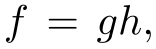
\includegraphics[width=43.75pt]{images-full/p124-i000.png}}\allowbreak{}，其中$g$ 与$h$ 首一，互素.又由于\allowbreak{}\raisebox{-3.00pt}{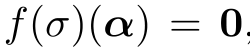
\includegraphics[width=70.30pt]{images-full/p124-i003.png}}\allowbreak{}，结合
\allowbreak{}\raisebox{-3.24pt}{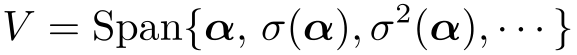
\includegraphics[width=162.72pt]{images-full/p124-i004.png}}\allowbreak{}可知\allowbreak{}\raisebox{-3.00pt}{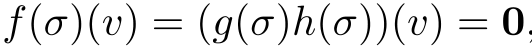
\includegraphics[width=149.99pt]{images-full/p124-i005.png}}\allowbreak{},\allowbreak{}\raisebox{-2.52pt}{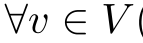
\includegraphics[width=40.13pt]{images-full/p124-i006.png}}\allowbreak{}因\allowbreak{}\raisebox{-1.56pt}{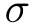
\includegraphics[width=10.17pt]{images-full/p124-i007.png}}\allowbreak{} 与\allowbreak{}\raisebox{-3.00pt}{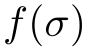
\includegraphics[width=25.42pt]{images-full/p124-i008.png}}\allowbreak{}
可换).故由例2.2.24 可知，$V$ 可分解为\allowbreak{}\raisebox{-3.00pt}{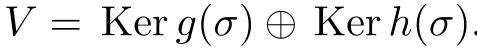
\includegraphics[width=134.33pt]{images-full/p124-i010.png}}\allowbreak{}
令\allowbreak{}\raisebox{-3.00pt}{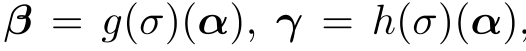
\includegraphics[width=148.25pt]{images-full/p124-i011.png}}\allowbreak{}，则断言:\allowbreak{}\raisebox{-2.88pt}{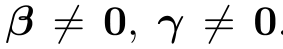
\includegraphics[width=79.49pt]{images-full/p124-i012.png}}\allowbreak{} 事实上，若\allowbreak{}\raisebox{-2.76pt}{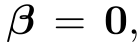
\includegraphics[width=38.73pt]{images-full/p124-i013.png}}\allowbreak{}，则由
\allowbreak{}\raisebox{-3.00pt}{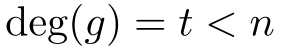
\includegraphics[width=79.10pt]{images-full/p124-i014.png}}\allowbreak{}可知\allowbreak{}\raisebox{-3.12pt}{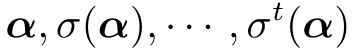
\includegraphics[width=99.44pt]{images-full/p124-i015.png}}\allowbreak{}线性相关，从丽由\allowbreak{}\raisebox{-3.36pt}{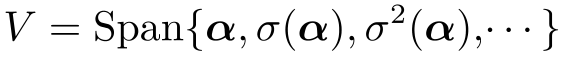
\includegraphics[width=159.33pt]{images-full/p124-i016.png}}\allowbreak{}
可知\allowbreak{}\raisebox{-2.76pt}{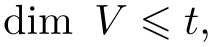
\includegraphics[width=60.45pt]{images-full/p124-i017.png}}\allowbreak{}与\allowbreak{}\raisebox{-2.28pt}{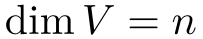
\includegraphics[width=57.06pt]{images-full/p124-i018.png}}\allowbreak{}矛盾.同理可知\allowbreak{}\raisebox{-2.76pt}{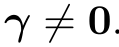
\includegraphics[width=33.10pt]{images-full/p124-i019.png}}\allowbreak{} 断言成立.
利用$g$ 与$h$ 互素，可取包\allowbreak{}\raisebox{-2.16pt}{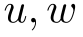
\includegraphics[width=23.16pt]{images-full/p124-i022.png}}\allowbreak{} 使得\allowbreak{}\raisebox{-2.76pt}{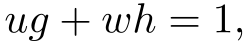
\includegraphics[width=69.00pt]{images-full/p124-i023.png}}\allowbreak{}其中包\allowbreak{}\raisebox{-3.00pt}{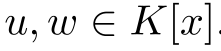
\includegraphics[width=61.96pt]{images-full/p124-i024.png}}\allowbreak{} 因此\allowbreak{}\raisebox{-1.68pt}{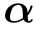
\includegraphics[width=11.30pt]{images-full/p124-i025.png}}\allowbreak{} 可分解为
\sourceblock{172.32}{images-full/p124-d000.png}
注意到\allowbreak{}\raisebox{-2.88pt}{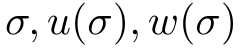
\includegraphics[width=67.80pt]{images-full/p124-i026.png}}\allowbreak{} 可交换，于是得
\sourceblock{307.36}{images-full/p124-d001.png}
最后，由\allowbreak{}\raisebox{-3.00pt}{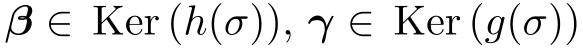
\includegraphics[width=164.41pt]{images-full/p124-i027.png}}\allowbreak{} 得
\sourceblock{382.50}{images-full/p124-d002.png}
\par 但.3真题选讲与点评\}-
\par\medskip\noindent\textbf{【例2.3.1 】(第十四届全国初赛题)设}
\sourceblock{231.65}{images-full/p124-d003.png}
\sourceblock{440.13}{images-full/p124-d004.png}


% SOURCE_PDF_PAGE 125

\hypertarget{source-p125}{}
\sourceblock{324.87}{images-full/p125-d000.png}
故$A$ 的特征值为\allowbreak{}\raisebox{-2.64pt}{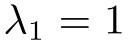
\includegraphics[width=36.16pt]{images-full/p125-i001.png}}\allowbreak{} (2 重)，\allowbreak{}\raisebox{-3.00pt}{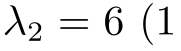
\includegraphics[width=50.85pt]{images-full/p125-i002.png}}\allowbreak{} 重).现在$A$ 可对角化，困此其每个特征值的
代数重数等于其儿何重数.故$A$ 的λ1 = 1 的特征子空间的维数为2. 由(A - >'tE)y = 0
\sourceblock{362.16}{images-full/p125-d001.png}
\sourceblock{281.37}{images-full/p125-d002.png}
\sourceblock{318.09}{images-full/p125-d003.png}


% SOURCE_PDF_PAGE 126

\hypertarget{source-p126}{}
\sourceblock{320.92}{images-full/p126-d000.png}
相应于情形(1) 得
\sourceblock{255.38}{images-full/p126-d001.png}
经检验知，本题所求的\allowbreak{}\raisebox{-2.16pt}{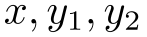
\includegraphics[width=41.24pt]{images-full/p126-i000.png}}\allowbreak{}共有三组解:
\sourceblock{445.22}{images-full/p126-d002.png}
【点评】本题考察的是相似矩阵的性质.一个关键点是需要掌握如何将一个循环矩
阵进行对角化.
\par\medskip\noindent\textbf{【例2.3.2】(第一届全国初赛题)设Mo.(C) 是\allowbreak{}\raisebox{-1.80pt}{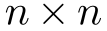
\includegraphics[width=29.94pt]{images-full/p126-i001.png}}\allowbreak{} 复矩阵全体在通常的运算下所}
\sourceblock{276.85}{images-full/p126-d003.png}
\par\noindent (1) 假设\allowbreak{}\raisebox{-3.12pt}{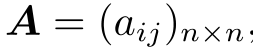
\includegraphics[width=71.18pt]{images-full/p126-i002.png}}\allowbreak{}，若\allowbreak{}\raisebox{-2.76pt}{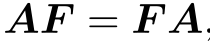
\includegraphics[width=59.18pt]{images-full/p126-i003.png}}\allowbreak{}，证明:
\sourceblock{258.77}{images-full/p126-d004.png}
\par\noindent (2) 求\allowbreak{}\raisebox{-3.00pt}{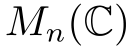
\includegraphics[width=37.29pt]{images-full/p126-i004.png}}\allowbreak{} 的子空间\allowbreak{}\raisebox{-3.00pt}{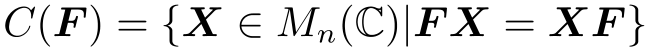
\includegraphics[width=183.62pt]{images-full/p126-i005.png}}\allowbreak{} 的维数


% SOURCE_PDF_PAGE 127

\hypertarget{source-p127}{}
\par\noindent (1) 证明将$A$ 列分块
\sourceblock{117.52}{images-full/p127-d000.png}
\sourceblock{359.90}{images-full/p127-d001.png}
\sourceblock{450.00}{images-full/p127-d002.png}
则\allowbreak{}\raisebox{-3.00pt}{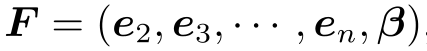
\includegraphics[width=120.23pt]{images-full/p127-i001.png}}\allowbreak{}，注意到
\sourceblock{433.35}{images-full/p127-d003.png}
由
\sourceblock{292.10}{images-full/p127-d004.png}
知
\sourceblock{290.41}{images-full/p127-d005.png}
\sourceblock{342.95}{images-full/p127-d006.png}
所以\allowbreak{}\raisebox{-2.28pt}{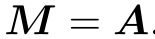
\includegraphics[width=43.52pt]{images-full/p127-i002.png}}\allowbreak{} 获证.口
\sourceblock{288.71}{images-full/p127-d007.png}
因此有\allowbreak{}\raisebox{-3.00pt}{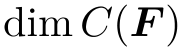
\includegraphics[width=51.98pt]{images-full/p127-i003.png}}\allowbreak{} 等于\allowbreak{}\raisebox{-3.24pt}{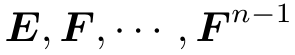
\includegraphics[width=83.05pt]{images-full/p127-i004.png}}\allowbreak{} 的秩.下面证明\allowbreak{}\raisebox{-3.24pt}{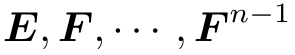
\includegraphics[width=83.05pt]{images-full/p127-i005.png}}\allowbreak{}线性无关.
设\allowbreak{}\raisebox{-3.12pt}{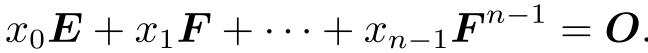
\includegraphics[width=182.69pt]{images-full/p127-i006.png}}\allowbreak{} 等式两边同时右乘\allowbreak{}\raisebox{-2.16pt}{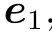
\includegraphics[width=14.25pt]{images-full/p127-i007.png}}\allowbreak{}利用(2.3.1) 式得
\sourceblock{250.29}{images-full/p127-d008.png}
则有\allowbreak{}\raisebox{-2.64pt}{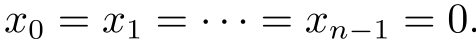
\includegraphics[width=133.95pt]{images-full/p127-i008.png}}\allowbreak{} 由此，直接得到\allowbreak{}\raisebox{-3.00pt}{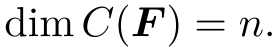
\includegraphics[width=76.44pt]{images-full/p127-i009.png}}\allowbreak{}


% SOURCE_PDF_PAGE 128

\hypertarget{source-p128}{}
【点评】此题的主要考点是求向量空间的维数.为此关键是要找出该空间的一个生
成系，进而从这个生成系中找出其最大无关组所含向量的个数.
\par\medskip\noindent\textbf{【例2.3.3) (第十二届全国决赛题(非数学类))设$A$ 是$n$ 阶实对称阵，证明:}
\par\noindent (1) 存在实对称阵$B$ 使得\allowbreak{}\raisebox{-3.12pt}{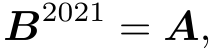
\includegraphics[width=59.89pt]{images-full/p128-i003.png}}\allowbreak{}且\allowbreak{}\raisebox{-2.76pt}{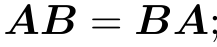
\includegraphics[width=60.99pt]{images-full/p128-i004.png}}\allowbreak{}
\par\noindent (2) 存在一个多项式\allowbreak{}\raisebox{-3.00pt}{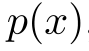
\includegraphics[width=24.94pt]{images-full/p128-i005.png}}\allowbreak{}，使得上述矩阵\allowbreak{}\raisebox{-3.00pt}{\includegraphics[width=54.41pt]{images-full/p128-i006.png}}\allowbreak{};
\par\noindent (3) 上述矩阵$B$ 是唯一的.
\par\noindent\textbf{证明}\ (1) 由$A$ 是实对称阵知z 存在正交矩阵$Q$ 使得
\sourceblock{156.50}{images-full/p128-d000.png}
其中\allowbreak{}\raisebox{-2.76pt}{\includegraphics[width=54.80pt]{images-full/p128-i010.png}}\allowbreak{} 为$A$ 的特征值，它们皆是实数.取
\sourceblock{204.53}{images-full/p128-d001.png}
\sourceblock{328.83}{images-full/p128-d002.png}
且AB=BA，得证.
\par\noindent (2) 设\allowbreak{}\raisebox{-2.64pt}{\includegraphics[width=54.24pt]{images-full/p128-i012.png}}\allowbreak{}为$A$ 的互不相同特征值，考虑以\allowbreak{}\raisebox{-2.04pt}{\includegraphics[width=80.79pt]{images-full/p128-i014.png}}\allowbreak{}为未知量的线性
方程组
\sourceblock{450.00}{images-full/p128-d003.png}
换.由于$B$与$C$均可对角化，困而存在可逆矩阵$P$ 使得
\sourceblock{176.84}{images-full/p128-d004.png}
\sourceblock{450.00}{images-full/p128-d005.png}


% SOURCE_PDF_PAGE 129

\hypertarget{source-p129}{}
【点评】此题充分应用实对称矩阵可对角化这一性质以及可换矩阵族有公共特征向
量这一结论来加以证明事实上，本题的本质属于矩阵函数范畴.
\par\medskip\noindent\textbf{【例2.3.4】(第一届全国决赛题)设\allowbreak{}\raisebox{-2.64pt}{\includegraphics[width=28.81pt]{images-full/p129-i000.png}}\allowbreak{} 均为\allowbreak{}\raisebox{-1.68pt}{\includegraphics[width=10.17pt]{images-full/p129-i001.png}}\allowbreak{} 阶半正定实对称矩阵，且满足}
\allowbreak{}\raisebox{-3.00pt}{\includegraphics[width=114.69pt]{images-full/p129-i002.png}}\allowbreak{} 证明:存在实可逆矩阵$C$使得\allowbreak{}\raisebox{-3.24pt}{\includegraphics[width=85.31pt]{images-full/p129-i004.png}}\allowbreak{} 皆为对角阵.
\par\noindent\textbf{证明}\ (1) \allowbreak{}\raisebox{-2.88pt}{\includegraphics[width=68.93pt]{images-full/p129-i005.png}}\allowbreak{} 的情形z 此时$A$ 正定，于是存在可逆矩阵$P$ 使得\allowbreak{}\raisebox{-2.76pt}{\includegraphics[width=52.54pt]{images-full/p129-i008.png}}\allowbreak{}
\allowbreak{}\raisebox{-3.24pt}{\includegraphics[width=59.32pt]{images-full/p129-i009.png}}\allowbreak{} 为实对称阵所以存在正交矩阵$Q$ 使得\allowbreak{}\raisebox{-3.60pt}{\includegraphics[width=83.62pt]{images-full/p129-i011.png}}\allowbreak{} 是对角阵令\allowbreak{}\raisebox{-2.40pt}{\includegraphics[width=25.42pt]{images-full/p129-i012.png}}\allowbreak{}
\allowbreak{}\raisebox{-2.76pt}{\includegraphics[width=23.21pt]{images-full/p129-i013.png}}\allowbreak{}，则\allowbreak{}\raisebox{-3.24pt}{\includegraphics[width=111.30pt]{images-full/p129-i014.png}}\allowbreak{} 都是对角阵.
\sourceblock{307.92}{images-full/p129-d000.png}
\sourceblock{137.86}{images-full/p129-d001.png}
\sourceblock{450.00}{images-full/p129-d002.png}
\sourceblock{354.82}{images-full/p129-d003.png}
\sourceblock{371.20}{images-full/p129-d004.png}
\sourceblock{185.32}{images-full/p129-d005.png}


% SOURCE_PDF_PAGE 130

\hypertarget{source-p130}{}
可同时合同于对角阵.
\sourceblock{450.00}{images-full/p130-d000.png}
\sourceblock{450.00}{images-full/p130-d001.png}
\sourceblock{313.57}{images-full/p130-d002.png}
\sourceblock{264.98}{images-full/p130-d003.png}


% SOURCE_PDF_PAGE 131

\hypertarget{source-p131}{}
\sourceblock{313.57}{images-full/p131-d000.png}
可同时合同于对角阵，进而$A$ 与$B$ 可合同于对角阵口
【点评】此题为两个矩阵同时合同对角化的问题.上述解答中在计算行列式
\sourceblock{169.50}{images-full/p131-d001.png}
时，可以不具体写出其表达式，只需知道它是一个关于$k$ 的多项式，其最高次项出现在
\allowbreak{}\raisebox{-3.00pt}{\includegraphics[width=120.34pt]{images-full/p131-i003.png}}\allowbreak{} 中即可.此时由于\allowbreak{}\raisebox{-2.76pt}{\includegraphics[width=31.60pt]{images-full/p131-i004.png}}\allowbreak{}，因而当$k$充分大时必定使该行列式\allowbreak{}\raisebox{-2.76pt}{\includegraphics[width=20.94pt]{images-full/p131-i006.png}}\allowbreak{}
\sourceblock{450.00}{images-full/p131-d002.png}
\sourceblock{139.55}{images-full/p131-d003.png}
不失一般性，可令
\sourceblock{287.02}{images-full/p131-d004.png}
\sourceblock{246.90}{images-full/p131-d005.png}
\sourceblock{159.89}{images-full/p131-d006.png}
\sourceblock{394.93}{images-full/p131-d007.png}
注意到
\sourceblock{272.33}{images-full/p131-d008.png}
故有\allowbreak{}\raisebox{-3.00pt}{\includegraphics[width=101.13pt]{images-full/p131-i007.png}}\allowbreak{}，即\allowbreak{}\raisebox{-2.64pt}{\includegraphics[width=69.35pt]{images-full/p131-i008.png}}\allowbreak{}
现在，\allowbreak{}\raisebox{-2.64pt}{\includegraphics[width=48.02pt]{images-full/p131-i009.png}}\allowbreak{}均可表示为\allowbreak{}\raisebox{-2.52pt}{\includegraphics[width=69.84pt]{images-full/p131-i010.png}}\allowbreak{}，其中\allowbreak{}\raisebox{-2.76pt}{\includegraphics[width=94.44pt]{images-full/p131-i011.png}}\allowbreak{} 此时
\sourceblock{183.06}{images-full/p131-d009.png}
\sourceblock{320.35}{images-full/p131-d010.png}


% SOURCE_PDF_PAGE 132

\hypertarget{source-p132}{}
【点评】此题的关键知识点有两个:一个是维数公式，另一个是齐次线性方程组的
解空间.解题思路清楚可见:就是首先将线性函数与其表示阵对应起来，然后利用齐次线
性方程组的解空间维数公式即可完成.
\par\medskip\noindent\textbf{【例2.3.61 (第二届全国决赛题)设\allowbreak{}\raisebox{-3.00pt}{\includegraphics[width=82.49pt]{images-full/p132-i000.png}}\allowbreak{} 是非零线性映射，满足}
\sourceblock{203.96}{images-full/p132-d000.png}
这里\allowbreak{}\raisebox{-3.00pt}{\includegraphics[width=37.29pt]{images-full/p132-i001.png}}\allowbreak{}表示实数域$R$上$n$ 阶方阵全体组成的实线性空间.在\allowbreak{}\raisebox{-3.00pt}{\includegraphics[width=37.29pt]{images-full/p132-i004.png}}\allowbreak{} 上定义双线性
型: \allowbreak{}\raisebox{-3.00pt}{\includegraphics[width=248.09pt]{images-full/p132-i005.png}}\allowbreak{}
\par\noindent (1) 证明: \allowbreak{}\raisebox{-3.00pt}{\includegraphics[width=22.60pt]{images-full/p132-i006.png}}\allowbreak{}，.)是非退化的，即若\allowbreak{}\raisebox{-3.00pt}{\includegraphics[width=61.16pt]{images-full/p132-i007.png}}\allowbreak{}，对\allowbreak{}\raisebox{-3.00pt}{\includegraphics[width=70.31pt]{images-full/p132-i008.png}}\allowbreak{}，则必然有\allowbreak{}\raisebox{-2.28pt}{\includegraphics[width=41.20pt]{images-full/p132-i009.png}}\allowbreak{}
\sourceblock{432.79}{images-full/p132-d001.png}
即
\sourceblock{154.24}{images-full/p132-d002.png}
\sourceblock{407.36}{images-full/p132-d003.png}
事实上，由题设知:\allowbreak{}\raisebox{-3.12pt}{\includegraphics[width=256.95pt]{images-full/p132-i010.png}}\allowbreak{}，其中\allowbreak{}\raisebox{-3.00pt}{\includegraphics[width=19.77pt]{images-full/p132-i011.png}}\allowbreak{} 是
\allowbreak{}\raisebox{-3.00pt}{\includegraphics[width=25.42pt]{images-full/p132-i012.png}}\allowbreak{}位置元为\allowbreak{}\raisebox{-2.52pt}{\includegraphics[width=10.73pt]{images-full/p132-i013.png}}\allowbreak{}，其余位置元为\allowbreak{}\raisebox{-2.28pt}{\includegraphics[width=8.47pt]{images-full/p132-i014.png}}\allowbreak{} 的矩阵.
令\allowbreak{}\raisebox{-2.88pt}{\includegraphics[width=62.57pt]{images-full/p132-i015.png}}\allowbreak{}则\allowbreak{}\raisebox{-3.12pt}{\includegraphics[width=109.24pt]{images-full/p132-i016.png}}\allowbreak{} ，故有\allowbreak{}\raisebox{-2.88pt}{\includegraphics[width=99.90pt]{images-full/p132-i017.png}}\allowbreak{}
\par\noindent (1) 显然，\allowbreak{}\raisebox{-3.00pt}{\includegraphics[width=22.03pt]{images-full/p132-i018.png}}\allowbreak{}，.)是双线性型，且是对称的.若\allowbreak{}\raisebox{-3.00pt}{\includegraphics[width=59.89pt]{images-full/p132-i019.png}}\allowbreak{} 对\allowbreak{}\raisebox{-3.00pt}{\includegraphics[width=70.62pt]{images-full/p132-i020.png}}\allowbreak{} 均成立，则
有\allowbreak{}\raisebox{-3.00pt}{\includegraphics[width=84.18pt]{images-full/p132-i021.png}}\allowbreak{} 对一切\allowbreak{}\raisebox{-3.00pt}{\includegraphics[width=62.71pt]{images-full/p132-i022.png}}\allowbreak{} 均成立.由$Y$ 的任意性，结合\allowbreak{}\raisebox{-3.00pt}{\includegraphics[width=67.80pt]{images-full/p132-i024.png}}\allowbreak{} 立即
\sourceblock{450.00}{images-full/p132-d004.png}


% SOURCE_PDF_PAGE 133

\hypertarget{source-p133}{}
\sourceblock{450.00}{images-full/p133-d000.png}
【点评】此题有一定的难度.破解此题的关键在于对迹函数的性质需要熟练掌握，
同时对对偶基的性质要能了然于心.本质上，此题的技巧常见于李代数这个分支中.从此
题也可看出，线性代数中那些在其他分支中有广泛应用的知识点，尤其经常作为考题的
内容.
\par\medskip\noindent\textbf{【例2.3.7】(第四届全国决赛题)设}
\sourceblock{450.00}{images-full/p133-d001.png}
\sourceblock{289.84}{images-full/p133-d002.png}
把\allowbreak{}\raisebox{-3.00pt}{\includegraphics[width=80.79pt]{images-full/p133-i000.png}}\allowbreak{})化为标准形.
解首先，
\sourceblock{337.87}{images-full/p133-d003.png}


% SOURCE_PDF_PAGE 134

\hypertarget{source-p134}{}
\sourceblock{183.62}{images-full/p134-d000.png}
其次，由\allowbreak{}\raisebox{-3.00pt}{\includegraphics[width=85.88pt]{images-full/p134-i002.png}}\allowbreak{}=  得\allowbreak{}\raisebox{-3.00pt}{\includegraphics[width=97.53pt]{images-full/p134-i003.png}}\allowbreak{}= ，即\allowbreak{}\raisebox{-3.00pt}{\includegraphics[width=80.82pt]{images-full/p134-i004.png}}\allowbreak{}=  故由\allowbreak{}\raisebox{-3.24pt}{\includegraphics[width=55.37pt]{images-full/p134-i005.png}}\allowbreak{}
由此可知:$f$ 为关于町\allowbreak{}\raisebox{-2.04pt}{\includegraphics[width=64.97pt]{images-full/p134-i001.png}}\allowbreak{}的二次型.
为\allowbreak{}\raisebox{-3.00pt}{\includegraphics[width=89.83pt]{images-full/p134-i006.png}}\allowbreak{} 的一个解知:$A$ 有特征值\allowbreak{}\raisebox{-2.28pt}{\includegraphics[width=17.31pt]{images-full/p134-i008.png}}\allowbreak{} 进一步，由条件\allowbreak{}\raisebox{-3.00pt}{\includegraphics[width=75.14pt]{images-full/p134-i009.png}}\allowbreak{} 的特
征值之和为\allowbreak{}\raisebox{-2.16pt}{\includegraphics[width=7.34pt]{images-full/p134-i010.png}}\allowbreak{}得到$A$ 的所有特征值:\allowbreak{}\raisebox{-2.76pt}{\includegraphics[width=40.05pt]{images-full/p134-i012.png}}\allowbreak{} 特征值\allowbreak{}\raisebox{-2.16pt}{\includegraphics[width=17.51pt]{images-full/p134-i013.png}}\allowbreak{}对应的特征子空间\allowbreak{}\raisebox{-2.64pt}{\includegraphics[width=20.90pt]{images-full/p134-i014.png}}\allowbreak{} 的维数
为1 ，特征值2 对应的特征子空间\allowbreak{}\raisebox{-2.64pt}{\includegraphics[width=14.12pt]{images-full/p134-i015.png}}\allowbreak{}的维数为2. 注意到\allowbreak{}\raisebox{-3.36pt}{\includegraphics[width=55.37pt]{images-full/p134-i016.png}}\allowbreak{} 是$A$ 对应于特征值
\sourceblock{358.21}{images-full/p134-d001.png}
\sourceblock{315.83}{images-full/p134-d002.png}
于是\allowbreak{}\raisebox{-2.76pt}{\includegraphics[width=38.42pt]{images-full/p134-i018.png}}\allowbreak{}作成\allowbreak{}\raisebox{-2.64pt}{\includegraphics[width=15.82pt]{images-full/p134-i019.png}}\allowbreak{}的标准正交基.令\allowbreak{}\raisebox{-3.00pt}{\includegraphics[width=73.55pt]{images-full/p134-i020.png}}\allowbreak{}，则有
\sourceblock{313.57}{images-full/p134-d003.png}


% SOURCE_PDF_PAGE 135

\hypertarget{source-p135}{}
\sourceblock{316.96}{images-full/p135-d000.png}
则有$Q$ 为正交阵，且在正交变换
\sourceblock{111.87}{images-full/p135-d001.png}
\sourceblock{306.23}{images-full/p135-d002.png}
\sourceblock{306.79}{images-full/p135-d003.png}
【点评】此题属将二次型化为标准形的综合题，主要侧重的是计算能力的考察.只
要对二次型的基本性质有较为系统的把握，就可做出-
['WIJ 2.3.8】(第五届全国决赛题)设\allowbreak{}\raisebox{-2.76pt}{\includegraphics[width=28.81pt]{images-full/p135-i001.png}}\allowbreak{} 皆为$n$ 阶实正定矩阵，求证:\allowbreak{}\raisebox{-2.28pt}{\includegraphics[width=23.16pt]{images-full/p135-i003.png}}\allowbreak{} 正定的
充要条件是\allowbreak{}\raisebox{-2.40pt}{\includegraphics[width=60.42pt]{images-full/p135-i004.png}}\allowbreak{}
\par\noindent\textbf{证明}\ 必要性\allowbreak{}\raisebox{-2.28pt}{\includegraphics[width=23.61pt]{images-full/p135-i005.png}}\allowbreak{} 正定表明\allowbreak{}\raisebox{-2.28pt}{\includegraphics[width=23.15pt]{images-full/p135-i006.png}}\allowbreak{} 是实对称阵.因此有\allowbreak{}\raisebox{-3.36pt}{\includegraphics[width=131.41pt]{images-full/p135-i007.png}}\allowbreak{},
即证.
充分性$A$ 正定，$B$iE.定，因此存在可逆阵\allowbreak{}\raisebox{-2.76pt}{\includegraphics[width=28.25pt]{images-full/p135-i010.png}}\allowbreak{} 使得\allowbreak{}\raisebox{-3.24pt}{\includegraphics[width=118.01pt]{images-full/p135-i011.png}}\allowbreak{}，进而
\allowbreak{}\raisebox{-3.24pt}{\includegraphics[width=94.26pt]{images-full/p135-i012.png}}\allowbreak{}. 则
\sourceblock{287.02}{images-full/p135-d004.png}


% SOURCE_PDF_PAGE 136

\hypertarget{source-p136}{}
注意到\allowbreak{}\raisebox{-3.24pt}{\includegraphics[width=29.94pt]{images-full/p136-i000.png}}\allowbreak{} 为可逆阵，因此\allowbreak{}\raisebox{-3.36pt}{\includegraphics[width=82.49pt]{images-full/p136-i001.png}}\allowbreak{} 为正定阵，从而\allowbreak{}\raisebox{-2.28pt}{\includegraphics[width=23.73pt]{images-full/p136-i002.png}}\allowbreak{} 的特征值为正数，
注意到$A$ 与$B$ 可交换肘，\allowbreak{}\raisebox{-2.28pt}{\includegraphics[width=23.16pt]{images-full/p136-i005.png}}\allowbreak{} 也是实对称的.故\allowbreak{}\raisebox{-2.28pt}{\includegraphics[width=23.73pt]{images-full/p136-i006.png}}\allowbreak{} 为正定阵口
【店、评】此题是关于正定矩阵判定问题的常规题目只需运用正定矩阵合同于单位
矩阵这一事实即可.
\par\medskip\noindent\textbf{【例2.3.91 (第九届全国决赛题(非数学类))设\allowbreak{}\raisebox{-3.24pt}{\includegraphics[width=141.25pt]{images-full/p136-i007.png}}\allowbreak{}，定义}
\sourceblock{192.10}{images-full/p136-d000.png}
\par\noindent (1) 证明:对一切非零\allowbreak{}\raisebox{-3.00pt}{\includegraphics[width=94.86pt]{images-full/p136-i008.png}}\allowbreak{}.
\par\noindent (2) 求\allowbreak{}\raisebox{-3.00pt}{\includegraphics[width=29.94pt]{images-full/p136-i009.png}}\allowbreak{} 满足条件\allowbreak{}\raisebox{-2.52pt}{\includegraphics[width=36.72pt]{images-full/p136-i010.png}}\allowbreak{} 的最小值.
\par\noindent (1) 证明\allowbreak{}\raisebox{-3.00pt}{\includegraphics[width=29.94pt]{images-full/p136-i011.png}}\allowbreak{} 为一个二次型，该二次型的矩阵为
\sourceblock{195.49}{images-full/p136-d001.png}
考察$A$ 的顺序主子式.直接计算可知
\sourceblock{87.57}{images-full/p136-d002.png}
故$A$ 正定，从而\allowbreak{}\raisebox{-3.00pt}{\includegraphics[width=29.94pt]{images-full/p136-i014.png}}\allowbreak{} 为正定二次型.口
\par\noindent (2) 解对$A$ 作如下分块:
\sourceblock{284.19}{images-full/p136-d003.png}
\sourceblock{149.16}{images-full/p136-d004.png}
\sourceblock{376.29}{images-full/p136-d005.png}
其中\allowbreak{}\raisebox{-3.48pt}{\includegraphics[width=98.42pt]{images-full/p136-i016.png}}\allowbreak{}


% SOURCE_PDF_PAGE 137

\hypertarget{source-p137}{}
\sourceblock{231.08}{images-full/p137-d000.png}
\sourceblock{375.16}{images-full/p137-d001.png}
\sourceblock{267.81}{images-full/p137-d002.png}
因为
\sourceblock{264.98}{images-full/p137-d003.png}
注意到\allowbreak{}\raisebox{-2.76pt}{\includegraphics[width=29.38pt]{images-full/p137-i000.png}}\allowbreak{}仍是正定矩阵，故
\sourceblock{424.88}{images-full/p137-d004.png}
\sourceblock{58.19}{images-full/p137-d005.png}
【点评】此题为二次型问题.值得指出的是，本题不但可求出\allowbreak{}\raisebox{-3.00pt}{\includegraphics[width=29.94pt]{images-full/p137-i001.png}}\allowbreak{} 在约束条件


% SOURCE_PDF_PAGE 138

\hypertarget{source-p138}{}
\allowbreak{}\raisebox{-2.64pt}{\includegraphics[width=36.72pt]{images-full/p138-i000.png}}\allowbreak{}下的最小值，还可求出\allowbreak{}\raisebox{-3.00pt}{\includegraphics[width=29.38pt]{images-full/p138-i001.png}}\allowbreak{} 在约束条件\allowbreak{}\raisebox{-2.64pt}{\includegraphics[width=36.72pt]{images-full/p138-i002.png}}\allowbreak{} 下的最小值点，它就是
\sourceblock{42.37}{images-full/p138-d000.png}
\par\medskip\noindent\textbf{【例2.3.10】(第十二届全国初赛题)假设$P$ 为对称国矩阵证明:存在可逆复矩阵}
$W$ 使得\allowbreak{}\raisebox{-2.76pt}{\includegraphics[width=70.45pt]{images-full/p138-i005.png}}\allowbreak{}•
\par\noindent\textbf{证明}\ $P$ 为西矩阵，自然为正规矩阵，故西相似对角化:存在国矩阵$U$ 使得
\sourceblock{189.84}{images-full/p138-d001.png}
其中\allowbreak{}\raisebox{-3.00pt}{\includegraphics[width=94.92pt]{images-full/p138-i008.png}}\allowbreak{} 均为模为1 的复数.取\allowbreak{}\raisebox{-3.00pt}{\includegraphics[width=94.35pt]{images-full/p138-i009.png}}\allowbreak{} 满足\allowbreak{}\raisebox{-3.24pt}{\includegraphics[width=43.03pt]{images-full/p138-i010.png}}\allowbreak{}并令
\sourceblock{298.32}{images-full/p138-d002.png}
\sourceblock{181.93}{images-full/p138-d003.png}
的系数行列式为Vandermonde 行列式且\allowbreak{}\raisebox{-2.88pt}{\includegraphics[width=21.78pt]{images-full/p138-i011.png}}\allowbreak{}，故有唯一解.因此，令\allowbreak{}\raisebox{-3.00pt}{\includegraphics[width=94.92pt]{images-full/p138-i012.png}}\allowbreak{}
\allowbreak{}\raisebox{-3.12pt}{\includegraphics[width=75.79pt]{images-full/p138-i013.png}}\allowbreak{}，则得
\sourceblock{202.27}{images-full/p138-d004.png}
\sourceblock{267.81}{images-full/p138-d005.png}


% SOURCE_PDF_PAGE 139

\hypertarget{source-p139}{}
现在$D$ 对称，$P$ 对称，\allowbreak{}\raisebox{-3.60pt}{\includegraphics[width=59.63pt]{images-full/p139-i002.png}}\allowbreak{}，所以
\sourceblock{249.16}{images-full/p139-d000.png}
\sourceblock{450.00}{images-full/p139-d001.png}
\sourceblock{294.36}{images-full/p139-d002.png}
故$Q$ 为西矩阵，且满足
\sourceblock{137.29}{images-full/p139-d003.png}
亦即\allowbreak{}\raisebox{-3.72pt}{\includegraphics[width=76.00pt]{images-full/p139-i004.png}}\allowbreak{} 若令\allowbreak{}\raisebox{-3.36pt}{\includegraphics[width=51.16pt]{images-full/p139-i005.png}}\allowbreak{}则有\allowbreak{}\raisebox{-2.76pt}{\includegraphics[width=70.85pt]{images-full/p139-i006.png}}\allowbreak{}•口
【点评】通常我们知道，实对称阵可正交相似于对角阵，特别地，半正走矩阵总可以
写成\allowbreak{}\raisebox{-2.76pt}{\includegraphics[width=33.90pt]{images-full/p139-i007.png}}\allowbreak{} 的形式.此题考察的是一个复对称阵的特殊情形:复对称西矩阵的结构问题.
此题中的结论在一些矩阵分析中可以见到.本题所用的知识是基本的，但技巧性较强.这
一点，只有平时多加练习，才能灵活掌握.
\par\medskip\noindent\textbf{【例2.3.11 】(第十三届全国决赛题)设矩阵\allowbreak{}\raisebox{-3.00pt}{\includegraphics[width=65.41pt]{images-full/p139-i008.png}}\allowbreak{}二元函数\allowbreak{}\raisebox{-3.00pt}{\includegraphics[width=46.33pt]{images-full/p139-i009.png}}\allowbreak{} 被}
定义为
\sourceblock{301.71}{images-full/p139-d004.png}
即\allowbreak{}\raisebox{-3.36pt}{\includegraphics[width=125.87pt]{images-full/p139-i010.png}}\allowbreak{}，其中\allowbreak{}\raisebox{-2.88pt}{\includegraphics[width=80.23pt]{images-full/p139-i011.png}}\allowbreak{} 为变量，\allowbreak{}\raisebox{-2.16pt}{\includegraphics[width=12.43pt]{images-full/p139-i012.png}}\allowbreak{} 表示矩阵的迹.现若$A$ 使
得\allowbreak{}\raisebox{-3.00pt}{\includegraphics[width=46.33pt]{images-full/p139-i014.png}}\allowbreak{} 成为实向量空间\allowbreak{}\raisebox{-3.00pt}{\includegraphics[width=36.16pt]{images-full/p139-i015.png}}\allowbreak{} 上的内积，并使得变换
\sourceblock{310.75}{images-full/p139-d005.png}


% SOURCE_PDF_PAGE 140

\hypertarget{source-p140}{}
成为此内积空间中的一个正交变换.求\allowbreak{}\raisebox{-2.28pt}{\includegraphics[width=12.05pt]{images-full/p140-i000.png}}\allowbreak{}
解(1) 易知，$p$ 为双线性函数，且有下列结论等价:
(i) $p$ 成为\allowbreak{}\raisebox{-3.00pt}{\includegraphics[width=36.16pt]{images-full/p140-i003.png}}\allowbreak{} 上的内积;
(ii) \allowbreak{}\raisebox{-3.00pt}{\includegraphics[width=70.06pt]{images-full/p140-i004.png}}\allowbreak{})有\allowbreak{}\raisebox{-3.00pt}{\includegraphics[width=69.84pt]{images-full/p140-i005.png}}\allowbreak{}，且\allowbreak{}\raisebox{-3.00pt}{\includegraphics[width=70.06pt]{images-full/p140-i006.png}}\allowbreak{} 当且仅当\allowbreak{}\raisebox{-2.76pt}{\includegraphics[width=40.78pt]{images-full/p140-i007.png}}\allowbreak{}
(iii) 二次型\allowbreak{}\raisebox{-3.36pt}{\includegraphics[width=161.59pt]{images-full/p140-i008.png}}\allowbreak{} 为正定二次型，其中
\sourceblock{100.00}{images-full/p140-d000.png}
现令
\sourceblock{363.86}{images-full/p140-d001.png}
直接计算可得
\sourceblock{380.81}{images-full/p140-d002.png}
因此
\sourceblock{155.37}{images-full/p140-d003.png}
\par\noindent (2) 在\allowbreak{}\raisebox{-3.00pt}{\includegraphics[width=46.33pt]{images-full/p140-i009.png}}\allowbreak{} 已成为\allowbreak{}\raisebox{-3.00pt}{\includegraphics[width=36.16pt]{images-full/p140-i010.png}}\allowbreak{} 上的内积的情况下，要使\allowbreak{}\raisebox{-1.56pt}{\includegraphics[width=9.60pt]{images-full/p140-i011.png}}\allowbreak{} 成为此内积下的正交变换，
当且仅当\allowbreak{}\raisebox{-1.68pt}{\includegraphics[width=9.60pt]{images-full/p140-i012.png}}\allowbreak{} 保持内积不变即可.因此又有
\sourceblock{242.95}{images-full/p140-d004.png}
\sourceblock{253.68}{images-full/p140-d005.png}


% SOURCE_PDF_PAGE 141

\hypertarget{source-p141}{}
于是直接计算可知
\sourceblock{450.00}{images-full/p141-d000.png}
比较\allowbreak{}\raisebox{-3.00pt}{\includegraphics[width=46.33pt]{images-full/p141-i000.png}}\allowbreak{} 与\allowbreak{}\raisebox{-3.00pt}{\includegraphics[width=79.10pt]{images-full/p141-i001.png}}\allowbreak{} 相应各项:比较\allowbreak{}\raisebox{-2.16pt}{\includegraphics[width=24.29pt]{images-full/p141-i002.png}}\allowbreak{}的系数可得\allowbreak{}\raisebox{-2.64pt}{\includegraphics[width=33.90pt]{images-full/p141-i003.png}}\allowbreak{} 比较\allowbreak{}\raisebox{-2.16pt}{\includegraphics[width=24.29pt]{images-full/p141-i004.png}}\allowbreak{}
的系数可得\allowbreak{}\raisebox{-2.40pt}{\includegraphics[width=38.56pt]{images-full/p141-i005.png}}\allowbreak{}
进一步可直接看出，在\allowbreak{}\raisebox{-2.28pt}{\includegraphics[width=32.20pt]{images-full/p141-i006.png}}\allowbreak{}且\allowbreak{}\raisebox{-2.28pt}{\includegraphics[width=39.55pt]{images-full/p141-i007.png}}\allowbreak{}条件下，\allowbreak{}\raisebox{-3.00pt}{\includegraphics[width=140.12pt]{images-full/p141-i008.png}}\allowbreak{} 己成为
恒等式.
\par\noindent (3) 故有所求的$A$ 为
\sourceblock{67.23}{images-full/p141-d001.png}
其中\allowbreak{}\raisebox{-2.76pt}{\includegraphics[width=41.24pt]{images-full/p141-i010.png}}\allowbreak{} 为任意实数.


% SOURCE_PDF_PAGE 142

\hypertarget{source-p142}{}
\par\medskip\noindent\textbf{【例2.3.12】(第十一届全国决赛题)设$V$ 为杳限维欧民空间，\allowbreak{}\raisebox{-2.64pt}{\includegraphics[width=30.51pt]{images-full/p142-i001.png}}\allowbreak{}为$V$ 的非平}
\sourceblock{450.00}{images-full/p142-d000.png}
正交.
\par\noindent\textbf{证明}\ 设\allowbreak{}\raisebox{-3.00pt}{\includegraphics[width=204.13pt]{images-full/p142-i003.png}}\allowbreak{} 分别取\allowbreak{}\raisebox{-2.64pt}{\includegraphics[width=30.51pt]{images-full/p142-i004.png}}\allowbreak{}的各一组标准正交
基，它们合起来得$V$ 的一组基.则\allowbreak{}\raisebox{-2.28pt}{\includegraphics[width=10.73pt]{images-full/p142-i006.png}}\allowbreak{}在这组基下的矩阵具有下列形式:
\sourceblock{110.17}{images-full/p142-d001.png}
\sourceblock{450.00}{images-full/p142-d002.png}
\sourceblock{120.34}{images-full/p142-d003.png}
由此得\allowbreak{}\raisebox{-2.88pt}{\includegraphics[width=46.74pt]{images-full/p142-i007.png}}\allowbreak{}. 进而\allowbreak{}\raisebox{-2.88pt}{\includegraphics[width=67.80pt]{images-full/p142-i008.png}}\allowbreak{} 为半正定矩阵，它就是\allowbreak{}\raisebox{-3.00pt}{\includegraphics[width=94.92pt]{images-full/p142-i009.png}}\allowbreak{}矩阵.
设\allowbreak{}\raisebox{-2.28pt}{\includegraphics[width=9.60pt]{images-full/p142-i010.png}}\allowbreak{} 为\allowbreak{}\raisebox{-3.00pt}{\includegraphics[width=37.85pt]{images-full/p142-i011.png}}\allowbreak{}的特征值(即\allowbreak{}\raisebox{-2.76pt}{\includegraphics[width=31.07pt]{images-full/p142-i012.png}}\allowbreak{} 的特征值)，\allowbreak{}\raisebox{-2.64pt}{\includegraphics[width=40.68pt]{images-full/p142-i013.png}}\allowbreak{}为P\allowbreak{}\raisebox{-3.00pt}{\includegraphics[width=40.68pt]{images-full/p142-i014.png}}\allowbreak{}关于\allowbreak{}\raisebox{-2.28pt}{\includegraphics[width=9.04pt]{images-full/p142-i015.png}}\allowbreak{} 的一个特
\sourceblock{450.00}{images-full/p142-d004.png}
\sourceblock{134.47}{images-full/p142-d005.png}
\sourceblock{336.17}{images-full/p142-d006.png}
最后，由上述推导可看出，\allowbreak{}\raisebox{-3.36pt}{\includegraphics[width=112.43pt]{images-full/p142-i016.png}}\allowbreak{} 的特征值均是\allowbreak{}\raisebox{-2.76pt}{\includegraphics[width=82.85pt]{images-full/p142-i017.png}}\allowbreak{} 由此得
\allowbreak{}\raisebox{-2.71pt}{\includegraphics[width=39.20pt]{images-full/p142-i018.png}}\allowbreak{}，进而\allowbreak{}\raisebox{-2.28pt}{\includegraphics[width=39.29pt]{images-full/p142-i019.png}}\allowbreak{}
所以，\allowbreak{}\raisebox{-2.88pt}{\includegraphics[width=89.27pt]{images-full/p142-i020.png}}\allowbreak{}与民\allowbreak{}\raisebox{-2.64pt}{\includegraphics[width=13.56pt]{images-full/p142-i021.png}}\allowbreak{}交.口
【点评】这是一道有关空间分解的试题.此题主要考察投影与正交投影的主要性质.
解题的关键在于掌握正交投影算子等价于其在标准正交基下的表示阵是自共辄罪等阵
在欧氏空间中，正交投影与对称军等阵相互对应.
\par\medskip\noindent\textbf{【例2.3.13】(第十二届全国初赛题)设\allowbreak{}\raisebox{-2.76pt}{\includegraphics[width=28.25pt]{images-full/p142-i022.png}}\allowbreak{} 均为2020 阶正交矩阵齐次线性方}
\sourceblock{448.04}{images-full/p142-d007.png}
解$A$一定不能相似于\allowbreak{}\raisebox{-2.28pt}{\includegraphics[width=12.76pt]{images-full/p142-i024.png}}\allowbreak{} 证明如下:
令\allowbreak{}\raisebox{-2.76pt}{\includegraphics[width=66.36pt]{images-full/p142-i025.png}}\allowbreak{} 则$C$ 仍是正交阵.把$C$ 看为百矩阵，于是存在可逆矩阵\allowbreak{}\raisebox{-2.76pt}{\includegraphics[width=13.41pt]{images-full/p142-i028.png}}\allowbreak{}S.t.
\allowbreak{}\raisebox{-3.12pt}{\includegraphics[width=71.43pt]{images-full/p142-i029.png}}\allowbreak{}，其中$D$ 为对角阵，主对角线元为$C$ 的2020 个特征值，它们均是模为1 的
复数. \allowbreak{}\raisebox{-2.40pt}{\includegraphics[width=54.80pt]{images-full/p142-i032.png}}\allowbreak{} 的解空间维数为3，即有\allowbreak{}\raisebox{-3.00pt}{\includegraphics[width=114.62pt]{images-full/p142-i033.png}}\allowbreak{} 进而
\sourceblock{308.49}{images-full/p142-d008.png}


% SOURCE_PDF_PAGE 143

\hypertarget{source-p143}{}
结果$D$ 中有3 个对角线元为1 其余主对角元均不为1.这表明$C$ 关于特征值1 的代数
重数为3. 注意到$C$是实矩阵，其复特征值共辄成对出现，$C$ 的阶2020 为偶数，$C$ 作为
正交矩阵，其实特征值不是\allowbreak{}\raisebox{-2.16pt}{\includegraphics[width=7.34pt]{images-full/p143-i005.png}}\allowbreak{}就是一\allowbreak{}\raisebox{-2.16pt}{\includegraphics[width=18.03pt]{images-full/p143-i006.png}}\allowbreak{}.故$C$ 必有\allowbreak{}\raisebox{-2.16pt}{\includegraphics[width=16.38pt]{images-full/p143-i008.png}}\allowbreak{}为特征值，且其代数重数也为奇数.
\sourceblock{316.40}{images-full/p143-d000.png}
特别地，\allowbreak{}\raisebox{-3.36pt}{\includegraphics[width=132.35pt]{images-full/p143-i009.png}}\allowbreak{}.故\allowbreak{}\raisebox{-2.76pt}{\includegraphics[width=96.05pt]{images-full/p143-i010.png}}\allowbreak{} 与$B$ 不可能相似.口
【点评】此题考察的一个知识点是:实系数多项式的复根要么为实数，要么共辄成
对出现.结合正交阵的实特征值要么为1，要么为\allowbreak{}\raisebox{-2.64pt}{\includegraphics[width=16.90pt]{images-full/p143-i012.png}}\allowbreak{}，由此便能得出解答.事实上，解答本
题中，若令\allowbreak{}\raisebox{-3.24pt}{\includegraphics[width=61.89pt]{images-full/p143-i013.png}}\allowbreak{}，同样可获得本题的答案，而思路则显得豆加自然.
<iJlJ 2.3.14】(第十二届全国决赛题)设$n$阶复方阵\allowbreak{}\raisebox{-2.76pt}{\includegraphics[width=87.01pt]{images-full/p143-i015.png}}\allowbreak{}均相似于对角
阵，\allowbreak{}\raisebox{-2.40pt}{\includegraphics[width=16.95pt]{images-full/p143-i016.png}}\allowbreak{} 表示复$n$ 维列向量空间.证明:
\sourceblock{450.00}{images-full/p143-d001.png}
\sourceblock{420.36}{images-full/p143-d002.png}
\sourceblock{180.23}{images-full/p143-d003.png}
\sourceblock{450.00}{images-full/p143-d004.png}
\sourceblock{263.29}{images-full/p143-d005.png}
\sourceblock{381.94}{images-full/p143-d006.png}
\sourceblock{144.07}{images-full/p143-d007.png}
\sourceblock{316.40}{images-full/p143-d008.png}


% SOURCE_PDF_PAGE 144

\hypertarget{source-p144}{}
又由\allowbreak{}\raisebox{-2.76pt}{\includegraphics[width=56.12pt]{images-full/p144-i000.png}}\allowbreak{}，故存在\allowbreak{}\raisebox{-2.40pt}{\includegraphics[width=41.06pt]{images-full/p144-i001.png}}\allowbreak{}，使得\allowbreak{}\raisebox{-2.76pt}{\includegraphics[width=53.34pt]{images-full/p144-i002.png}}\allowbreak{} 将$w$ 写成
\sourceblock{176.28}{images-full/p144-d000.png}
则得
\sourceblock{390.41}{images-full/p144-d001.png}
再次由\allowbreak{}\raisebox{-3.72pt}{\includegraphics[width=91.53pt]{images-full/p144-i004.png}}\allowbreak{} 是线性无关向量组，得\allowbreak{}\raisebox{-2.64pt}{\includegraphics[width=129.23pt]{images-full/p144-i005.png}}\allowbreak{}，从而\allowbreak{}\raisebox{-2.28pt}{\includegraphics[width=36.96pt]{images-full/p144-i006.png}}\allowbreak{}.
困此
\sourceblock{119.21}{images-full/p144-d002.png}
获证.
\par\noindent (2) 由(1) 知
\sourceblock{249.16}{images-full/p144-d003.png}
断言:\allowbreak{}\raisebox{-2.64pt}{\includegraphics[width=37.29pt]{images-full/p144-i007.png}}\allowbreak{} 可分解为
\sourceblock{201.14}{images-full/p144-d004.png}
事实上，\allowbreak{}\raisebox{-2.64pt}{\includegraphics[width=59.32pt]{images-full/p144-i008.png}}\allowbreak{}蕴含\allowbreak{}\raisebox{-2.64pt}{\includegraphics[width=86.43pt]{images-full/p144-i009.png}}\allowbreak{}•
\allowbreak{}\raisebox{-2.76pt}{\includegraphics[width=84.65pt]{images-full/p144-i010.png}}\allowbreak{} 可分解为\allowbreak{}\raisebox{-2.76pt}{\includegraphics[width=56.03pt]{images-full/p144-i011.png}}\allowbreak{}其中\allowbreak{}\raisebox{-2.88pt}{\includegraphics[width=121.59pt]{images-full/p144-i012.png}}\allowbreak{}. 则
\par \allowbreak{}\raisebox{-2.76pt}{\includegraphics[width=106.22pt]{images-full/p144-i013.png}}\allowbreak{}(锢因为\allowbreak{}\raisebox{-3.00pt}{\includegraphics[width=93.15pt]{images-full/p144-i014.png}}\allowbreak{}
进而\allowbreak{}\raisebox{-2.76pt}{\includegraphics[width=115.17pt]{images-full/p144-i015.png}}\allowbreak{}，从而\allowbreak{}\raisebox{-3.00pt}{\includegraphics[width=199.33pt]{images-full/p144-i016.png}}\allowbreak{} 断言真.
由断言知，\allowbreak{}\raisebox{-2.40pt}{\includegraphics[width=16.95pt]{images-full/p144-i017.png}}\allowbreak{} 有分解: \allowbreak{}\raisebox{-2.88pt}{\includegraphics[width=223.15pt]{images-full/p144-i018.png}}\allowbreak{}
利用\allowbreak{}\raisebox{-2.76pt}{\includegraphics[width=123.73pt]{images-full/p144-i019.png}}\allowbreak{} 及\allowbreak{}\raisebox{-2.76pt}{\includegraphics[width=116.25pt]{images-full/p144-i020.png}}\allowbreak{}，重复前述关于\allowbreak{}\raisebox{-2.76pt}{\includegraphics[width=37.85pt]{images-full/p144-i021.png}}\allowbreak{} 的分
解过程可得
\sourceblock{304.53}{images-full/p144-d005.png}
\sourceblock{370.07}{images-full/p144-d006.png}
\sourceblock{405.67}{images-full/p144-d007.png}
\sourceblock{342.95}{images-full/p144-d008.png}
因此\allowbreak{}\raisebox{-3.00pt}{\includegraphics[width=131.64pt]{images-full/p144-i022.png}}\allowbreak{})中至少有$n$ 个为0，亦即\allowbreak{}\raisebox{-2.76pt}{\includegraphics[width=87.01pt]{images-full/p144-i024.png}}\allowbreak{} 中至少有\allowbreak{}\raisebox{-1.68pt}{\includegraphics[width=9.60pt]{images-full/p144-i025.png}}\allowbreak{}个
矩阵为零矩阵口
【点评】此题实际上是一道关于空间的直和分解的题，解题的关键是在题设条件下
子空间在直和分解式中关于交的分配律成立.


% SOURCE_PDF_PAGE 145

\hypertarget{source-p145}{}
\par\medskip\noindent\textbf{【例2.3.15】(第一届全国初赛题)设$V$ 是复数域$C$上$n$维线性空间\allowbreak{}\raisebox{-3.00pt}{\includegraphics[width=64.97pt]{images-full/p145-i003.png}}\allowbreak{}}
为$V$ 上的线性变换.若\allowbreak{}\raisebox{-2.76pt}{\includegraphics[width=67.01pt]{images-full/p145-i005.png}}\allowbreak{} 证明:\allowbreak{}\raisebox{-2.76pt}{\includegraphics[width=9.60pt]{images-full/p145-i006.png}}\allowbreak{} 的特征值都是\allowbreak{}\raisebox{-2.64pt}{\includegraphics[width=8.89pt]{images-full/p145-i007.png}}\allowbreak{}，且\allowbreak{}\raisebox{-2.76pt}{\includegraphics[width=20.34pt]{images-full/p145-i008.png}}\allowbreak{} 有公共特征向量.
\par\noindent\textbf{证明}\ 设\allowbreak{}\raisebox{-2.28pt}{\includegraphics[width=9.60pt]{images-full/p145-i009.png}}\allowbreak{} 是$f$ 的特征值，$W$ 是相应特征子空间.则$W$ 是$f$ 的不变子空间.下证
\allowbreak{}\raisebox{-2.88pt}{\includegraphics[width=111.06pt]{images-full/p145-i014.png}}\allowbreak{}记$m$ 为使得\allowbreak{}\raisebox{-3.00pt}{\includegraphics[width=97.74pt]{images-full/p145-i016.png}}\allowbreak{} 线性相关的最小的非负整数.即，
当\allowbreak{}\raisebox{-2.52pt}{\includegraphics[width=74.58pt]{images-full/p145-i017.png}}\allowbreak{}时，\allowbreak{}\raisebox{-3.24pt}{\includegraphics[width=94.92pt]{images-full/p145-i018.png}}\allowbreak{} 线性无关.
令\allowbreak{}\raisebox{-3.24pt}{\includegraphics[width=218.60pt]{images-full/p145-i019.png}}\allowbreak{} 则有
\sourceblock{246.34}{images-full/p145-d000.png}
显见，\allowbreak{}\raisebox{-3.00pt}{\includegraphics[width=121.59pt]{images-full/p145-i020.png}}\allowbreak{}故\allowbreak{}\raisebox{-2.64pt}{\includegraphics[width=21.47pt]{images-full/p145-i021.png}}\allowbreak{} 是$g$ 的不变子空间.
此外，由\allowbreak{}\raisebox{-3.00pt}{\includegraphics[width=57.06pt]{images-full/p145-i023.png}}\allowbreak{} 知
\sourceblock{194.36}{images-full/p145-d001.png}
\sourceblock{429.40}{images-full/p145-d002.png}
根据
\sourceblock{310.75}{images-full/p145-d003.png}
困而用数学归纳法不难证明: \allowbreak{}\raisebox{-3.36pt}{\includegraphics[width=37.29pt]{images-full/p145-i024.png}}\allowbreak{} 一定可以表示为
\sourceblock{450.00}{images-full/p145-d004.png}
立即得\allowbreak{}\raisebox{-2.28pt}{\includegraphics[width=31.17pt]{images-full/p145-i025.png}}\allowbreak{}
最后，由\allowbreak{}\raisebox{-3.00pt}{\includegraphics[width=193.88pt]{images-full/p145-i026.png}}\allowbreak{} 困此\allowbreak{}\raisebox{-2.88pt}{\includegraphics[width=54.08pt]{images-full/p145-i027.png}}\allowbreak{} 因此，$W$ 在$g$ 下是
不变的，从而在$W$ 中存在$g$ 的特征向量\allowbreak{}\raisebox{-2.76pt}{\includegraphics[width=11.56pt]{images-full/p145-i032.png}}\allowbreak{}这也是$f$ 与$g$ 的公共特征向量.口
【点评】此题某种意义上可看成\allowbreak{}\raisebox{-2.28pt}{\includegraphics[width=16.95pt]{images-full/p145-i035.png}}\allowbreak{} 中两个可交换线性变换有公共特征向量这一
结果的推广.有一定的难度.解题的关键在于找出子空间有限升链:\allowbreak{}\raisebox{-3.36pt}{\includegraphics[width=99.44pt]{images-full/p145-i036.png}}\allowbreak{}
\allowbreak{}\raisebox{-2.76pt}{\includegraphics[width=147.46pt]{images-full/p145-i037.png}}\allowbreak{}.类似的技巧还经常用在将矩阵相似化简为具有某种特殊形
状的矩阵中，见下例.
\par\medskip\noindent\textbf{【例2.3.16】(第三届全国初赛题)设$A$ 是数域$F$上的$n$ 阶方阵.证明:$A$ 在数域}
\sourceblock{309.05}{images-full/p145-d005.png}
\par\noindent\textbf{证明}\ 把A 看成是域F 上的n 维向量些间V 上的线性变换σ. 下面证明存在σ-不
\sourceblock{362.16}{images-full/p145-d006.png}
考察子空间升链
\sourceblock{118.65}{images-full/p145-d007.png}


% SOURCE_PDF_PAGE 146

\hypertarget{source-p146}{}
\sourceblock{450.00}{images-full/p146-d000.png}
\allowbreak{}\raisebox{-3.12pt}{\includegraphics[width=50.44pt]{images-full/p146-i000.png}}\allowbreak{} 从而
\sourceblock{349.73}{images-full/p146-d001.png}
特别地，\allowbreak{}\raisebox{-2.76pt}{\includegraphics[width=97.74pt]{images-full/p146-i001.png}}\allowbreak{}
下证: \allowbreak{}\raisebox{-2.52pt}{\includegraphics[width=111.49pt]{images-full/p146-i002.png}}\allowbreak{}
首先，\allowbreak{}\raisebox{-2.40pt}{\includegraphics[width=114.06pt]{images-full/p146-i003.png}}\allowbreak{}，则由\allowbreak{}\raisebox{-2.40pt}{\includegraphics[width=55.37pt]{images-full/p146-i004.png}}\allowbreak{} 知:存在\allowbreak{}\raisebox{-2.76pt}{\includegraphics[width=35.26pt]{images-full/p146-i005.png}}\allowbreak{}，使得\allowbreak{}\raisebox{-2.76pt}{\includegraphics[width=51.32pt]{images-full/p146-i006.png}}\allowbreak{}. 故有
\sourceblock{236.73}{images-full/p146-d002.png}
从而\allowbreak{}\raisebox{-2.76pt}{\includegraphics[width=73.86pt]{images-full/p146-i007.png}}\allowbreak{} 因此\allowbreak{}\raisebox{-2.28pt}{\includegraphics[width=38.98pt]{images-full/p146-i008.png}}\allowbreak{} 与\allowbreak{}\raisebox{-2.28pt}{\includegraphics[width=32.20pt]{images-full/p146-i009.png}}\allowbreak{} 的和是直和.此外，
\sourceblock{392.11}{images-full/p146-d003.png}
故有\allowbreak{}\raisebox{-2.52pt}{\includegraphics[width=110.32pt]{images-full/p146-i010.png}}\allowbreak{}进一步地，\allowbreak{}\raisebox{-2.64pt}{\includegraphics[width=83.35pt]{images-full/p146-i011.png}}\allowbreak{} 记\allowbreak{}\raisebox{-2.76pt}{\includegraphics[width=133.60pt]{images-full/p146-i012.png}}\allowbreak{}直
接检验可知\allowbreak{}\raisebox{-2.64pt}{\includegraphics[width=31.07pt]{images-full/p146-i013.png}}\allowbreak{}均是\allowbreak{}\raisebox{-1.68pt}{\includegraphics[width=11.23pt]{images-full/p146-i014.png}}\allowbreak{}不变子些间.性意到\allowbreak{}\raisebox{-3.00pt}{\includegraphics[width=99.13pt]{images-full/p146-i015.png}}\allowbreak{}，故有\allowbreak{}\raisebox{-3.00pt}{\includegraphics[width=25.99pt]{images-full/p146-i016.png}}\allowbreak{}是军零变
换.又由\allowbreak{}\raisebox{-2.76pt}{\includegraphics[width=83.62pt]{images-full/p146-i017.png}}\allowbreak{}知σ|巧是满线性映射，从而是同构.现在取民的一组基并上
\sourceblock{450.00}{images-full/p146-d004.png}
【点评】此题属于把矩阵看成线性变换来进行处理的典型例子. 细心的读者甚至会
发现，此题在P. Halmos 著的《有限维向量空间》一书中有相应的描述和推导，这里我
们就不细讲了.高等代数中，把矩阵视为有限维空间中的线性变换，从而通过几何性态的
研究来解剖矩阵的代数性质，是一个十分重要的知识点，也必是高等代数命题的长期话题
之一.
\par\medskip\noindent\textbf{【例2.3.17】(第十五届全国初赛题)设$V$ 是复数域$C$上的$n$维线性空间，$A$ 是$V$}
上的一个线性变换.证明:存在\allowbreak{}\raisebox{-2.28pt}{\includegraphics[width=36.16pt]{images-full/p146-i023.png}}\allowbreak{} 使得\allowbreak{}\raisebox{-3.36pt}{\includegraphics[width=109.61pt]{images-full/p146-i024.png}}\allowbreak{} 成为$V$ 的一组基当且
仅当对于$A$ 的任一特征值\allowbreak{}\raisebox{-2.76pt}{\includegraphics[width=23.73pt]{images-full/p146-i027.png}}\allowbreak{} 的几何重数为1.
\par\noindent\textbf{证明}\ 必要性设存在\allowbreak{}\raisebox{-2.40pt}{\includegraphics[width=35.59pt]{images-full/p146-i028.png}}\allowbreak{} 使得\allowbreak{}\raisebox{-3.24pt}{\includegraphics[width=109.61pt]{images-full/p146-i029.png}}\allowbreak{} 成为$V$ 的一组基，显然$A$
\sourceblock{302.27}{images-full/p146-d005.png}


% SOURCE_PDF_PAGE 147

\hypertarget{source-p147}{}
\sourceblock{307.36}{images-full/p147-d000.png}
其左下角的\allowbreak{}\raisebox{-2.16pt}{\includegraphics[width=29.94pt]{images-full/p147-i000.png}}\allowbreak{}阶子式非霉，所以\allowbreak{}\raisebox{-3.00pt}{\includegraphics[width=118.99pt]{images-full/p147-i001.png}}\allowbreak{}，从而齐次线性方程组
\sourceblock{81.92}{images-full/p147-d001.png}
\sourceblock{207.35}{images-full/p147-d002.png}
又对$A$ 的任一特征值\allowbreak{}\raisebox{-2.76pt}{\includegraphics[width=9.49pt]{images-full/p147-i003.png}}\allowbreak{}，
\sourceblock{83.62}{images-full/p147-d003.png}
一定有非零解，它的解空间维数\allowbreak{}\raisebox{-2.52pt}{\includegraphics[width=20.49pt]{images-full/p147-i004.png}}\allowbreak{}.所以齐次线性方程组
\sourceblock{83.62}{images-full/p147-d004.png}
的解空间维数为1 ，即\allowbreak{}\raisebox{-2.28pt}{\includegraphics[width=9.04pt]{images-full/p147-i005.png}}\allowbreak{} 的几何重数为1.
充分性设$A$ 的互不相同的特征值为\allowbreak{}\raisebox{-2.76pt}{\includegraphics[width=73.39pt]{images-full/p147-i007.png}}\allowbreak{}，代数重数分别为\allowbreak{}\raisebox{-2.76pt}{\includegraphics[width=69.53pt]{images-full/p147-i008.png}}\allowbreak{}，
\sourceblock{263.29}{images-full/p147-d005.png}
\sourceblock{218.09}{images-full/p147-d006.png}
对于\allowbreak{}\raisebox{-2.52pt}{\includegraphics[width=49.29pt]{images-full/p147-i009.png}}\allowbreak{}，记\allowbreak{}\raisebox{-3.36pt}{\includegraphics[width=113.02pt]{images-full/p147-i010.png}}\allowbreak{}，其中1 为恒等变换，则\allowbreak{}\raisebox{-2.88pt}{\includegraphics[width=17.51pt]{images-full/p147-i011.png}}\allowbreak{}为\allowbreak{}\raisebox{-2.28pt}{\includegraphics[width=16.02pt]{images-full/p147-i012.png}}\allowbreak{}不变子些问且
\sourceblock{138.99}{images-full/p147-d007.png}
由于\allowbreak{}\raisebox{-2.64pt}{\includegraphics[width=12.43pt]{images-full/p147-i013.png}}\allowbreak{}的几何重数为1，故\allowbreak{}\raisebox{-3.36pt}{\includegraphics[width=28.81pt]{images-full/p147-i014.png}}\allowbreak{}的Jordan 标准形为
\sourceblock{143.51}{images-full/p147-d008.png}
所以存在\allowbreak{}\raisebox{-2.88pt}{\includegraphics[width=45.20pt]{images-full/p147-i015.png}}\allowbreak{}使得\allowbreak{}\raisebox{-3.24pt}{\includegraphics[width=112.45pt]{images-full/p147-i016.png}}\allowbreak{}
令
\sourceblock{129.95}{images-full/p147-d009.png}


% SOURCE_PDF_PAGE 148

\hypertarget{source-p148}{}
\phantomsection\addcontentsline{toc}{section}{2.4 能力拓展与训练}
则\allowbreak{}\raisebox{-3.48pt}{\includegraphics[width=112.43pt]{images-full/p148-i000.png}}\allowbreak{} 是$V$ 的一组基.若否，则\allowbreak{}\raisebox{-3.24pt}{\includegraphics[width=101.13pt]{images-full/p148-i002.png}}\allowbreak{} 线性相关，从而存
在次数\allowbreak{}\raisebox{-2.52pt}{\includegraphics[width=41.81pt]{images-full/p148-i003.png}}\allowbreak{}的非零多项式\allowbreak{}\raisebox{-3.00pt}{\includegraphics[width=61.02pt]{images-full/p148-i004.png}}\allowbreak{}使得\allowbreak{}\raisebox{-3.00pt}{\includegraphics[width=60.22pt]{images-full/p148-i005.png}}\allowbreak{} 由于\allowbreak{}\raisebox{-2.88pt}{\includegraphics[width=16.95pt]{images-full/p148-i006.png}}\allowbreak{}为$A$-不变子空间，
所以\allowbreak{}\raisebox{-3.00pt}{\includegraphics[width=73.14pt]{images-full/p148-i008.png}}\allowbreak{}由
\sourceblock{250.29}{images-full/p148-d000.png}
可知\allowbreak{}\raisebox{-3.00pt}{\includegraphics[width=64.36pt]{images-full/p148-i009.png}}\allowbreak{} 由于\allowbreak{}\raisebox{-3.36pt}{\includegraphics[width=111.68pt]{images-full/p148-i010.png}}\allowbreak{}，所以\allowbreak{}\raisebox{-3.36pt}{\includegraphics[width=49.72pt]{images-full/p148-i011.png}}\allowbreak{}是$A$ 的零化\allowbreak{}\raisebox{-2.04pt}{\includegraphics[width=14.69pt]{images-full/p148-i013.png}}\allowbreak{}的次数最
\sourceblock{272.33}{images-full/p148-d001.png}
又当\allowbreak{}\raisebox{-2.76pt}{\includegraphics[width=27.68pt]{images-full/p148-i014.png}}\allowbreak{} 时，\allowbreak{}\raisebox{-3.36pt}{\includegraphics[width=50.85pt]{images-full/p148-i015.png}}\allowbreak{}与\allowbreak{}\raisebox{-3.48pt}{\includegraphics[width=51.98pt]{images-full/p148-i016.png}}\allowbreak{}互素，所以
\sourceblock{210.74}{images-full/p148-d002.png}
即\allowbreak{}\raisebox{-3.00pt}{\includegraphics[width=57.28pt]{images-full/p148-i017.png}}\allowbreak{}，这与\allowbreak{}\raisebox{-3.00pt}{\includegraphics[width=102.83pt]{images-full/p148-i018.png}}\allowbreak{} 且\allowbreak{}\raisebox{-3.00pt}{\includegraphics[width=46.89pt]{images-full/p148-i019.png}}\allowbreak{}矛盾.口
\sourceblock{320.92}{images-full/p148-d003.png}
\sourceblock{310.75}{images-full/p148-d004.png}
\sourceblock{294.36}{images-full/p148-d005.png}
\allowbreak{}\raisebox{-2.76pt}{\includegraphics[width=66.05pt]{images-full/p148-i020.png}}\allowbreak{}，试求$f$在正交变换下的标准形.
2. 设\allowbreak{}\raisebox{-2.76pt}{\includegraphics[width=44.63pt]{images-full/p148-i022.png}}\allowbreak{} 均为$n$ 阶复方阵，且满足\allowbreak{}\raisebox{-2.76pt}{\includegraphics[width=213.42pt]{images-full/p148-i024.png}}\allowbreak{}
\par\noindent (1) 证明:$C$是军军阵.
\par\noindent (2) 证明:\allowbreak{}\raisebox{-2.76pt}{\includegraphics[width=45.20pt]{images-full/p148-i026.png}}\allowbreak{}能同时相似于上三角阵.
\sourceblock{450.00}{images-full/p148-d006.png}
的值.
4. 设$A$ 为实对称矩阵，\allowbreak{}\raisebox{-3.00pt}{\includegraphics[width=38.98pt]{images-full/p148-i028.png}}\allowbreak{} 和\allowbreak{}\raisebox{-3.00pt}{\includegraphics[width=38.42pt]{images-full/p148-i029.png}}\allowbreak{} 构成其行向量的一个极大无关组，求\allowbreak{}\raisebox{-2.28pt}{\includegraphics[width=12.16pt]{images-full/p148-i030.png}}\allowbreak{}


% SOURCE_PDF_PAGE 149

\hypertarget{source-p149}{}
5. 证明:任意$n$阶实方阵$A$ 可以分解成\allowbreak{}\raisebox{-2.76pt}{\includegraphics[width=99.49pt]{images-full/p149-i002.png}}\allowbreak{}其中\allowbreak{}\raisebox{-2.76pt}{\includegraphics[width=91.04pt]{images-full/p149-i003.png}}\allowbreak{}
\allowbreak{}\raisebox{-2.64pt}{\includegraphics[width=16.95pt]{images-full/p149-i004.png}}\allowbreak{}与\allowbreak{}\raisebox{-2.64pt}{\includegraphics[width=16.95pt]{images-full/p149-i005.png}}\allowbreak{}都是罪零方阵
6. 设实二次型\allowbreak{}\raisebox{-3.36pt}{\includegraphics[width=130.50pt]{images-full/p149-i006.png}}\allowbreak{}，其中
\sourceblock{224.87}{images-full/p149-d000.png}
\allowbreak{}\raisebox{-2.88pt}{\includegraphics[width=115.82pt]{images-full/p149-i007.png}}\allowbreak{} 皆为实数，己知\allowbreak{}\raisebox{-2.64pt}{\includegraphics[width=36.16pt]{images-full/p149-i008.png}}\allowbreak{} 是$A$ 的一个几何重数为3 的特征值.试回
答以下问题:
\par\noindent (1) $A$ 能否相似于对角阵若能，请给出证明;若不能，请给出例子.
\par\noindent (2) 当\allowbreak{}\raisebox{-2.52pt}{\includegraphics[width=35.59pt]{images-full/p149-i011.png}}\allowbreak{} 时，试求\allowbreak{}\raisebox{-3.00pt}{\includegraphics[width=80.79pt]{images-full/p149-i012.png}}\allowbreak{} 在正交变换下的标准形.
7. 设π 阶实方阵
\sourceblock{450.00}{images-full/p149-d001.png}
\allowbreak{}\raisebox{-3.00pt}{\includegraphics[width=29.90pt]{images-full/p149-i013.png}}\allowbreak{}，证明$W$ 是$R$上的向量塑间，且\allowbreak{}\raisebox{-3.24pt}{\includegraphics[width=83.62pt]{images-full/p149-i016.png}}\allowbreak{} 为其一组基，其中$E$ 为$n$ 阶单
位阵
8. 将实2024 阶对称阵按合同关系进行分类，即两个实2024 阶对称阵属于同一类，
当且仅当它们相互合同.问其有多少类?
9. 己知实二次型
\sourceblock{272.89}{images-full/p149-d002.png}
求f 的规范形.
1 1.设\allowbreak{}\raisebox{-2.76pt}{\includegraphics[width=30.51pt]{images-full/p149-i019.png}}\allowbreak{} 皆为正定矩阵，证明\allowbreak{}\raisebox{-2.28pt}{\includegraphics[width=23.16pt]{images-full/p149-i020.png}}\allowbreak{} 的全部特征值皆大于\allowbreak{}\raisebox{-2.28pt}{\includegraphics[width=8.49pt]{images-full/p149-i021.png}}\allowbreak{}


% SOURCE_PDF_PAGE 150

\hypertarget{source-p150}{}
12.设$A$ 为$n$ 阶实对称矩阵证明: \allowbreak{}\raisebox{-3.00pt}{\includegraphics[width=72.88pt]{images-full/p150-i002.png}}\allowbreak{} 当且仅当存在实矩阵$B$ 使得
\allowbreak{}\raisebox{-2.88pt}{\includegraphics[width=66.67pt]{images-full/p150-i004.png}}\allowbreak{} 是正定矩阵.
13. 设\allowbreak{}\raisebox{-2.16pt}{\includegraphics[width=70.62pt]{images-full/p150-i005.png}}\allowbreak{} 是和为\allowbreak{}\raisebox{-2.16pt}{\includegraphics[width=7.34pt]{images-full/p150-i006.png}}\allowbreak{} 的\allowbreak{}\raisebox{-1.68pt}{\includegraphics[width=9.60pt]{images-full/p150-i007.png}}\allowbreak{}个正数，\allowbreak{}\raisebox{-3.12pt}{\includegraphics[width=70.62pt]{images-full/p150-i008.png}}\allowbreak{} 为$n$ 阶方阵，其每一行均
是\allowbreak{}\raisebox{-2.04pt}{\includegraphics[width=70.62pt]{images-full/p150-i010.png}}\allowbreak{}的一个排列.
\par\noindent (1) 证明:1 是$A$ 的特征值;
\par\noindent (2) 设\allowbreak{}\raisebox{-2.64pt}{\includegraphics[width=12.99pt]{images-full/p150-i012.png}}\allowbreak{} 表示$A$ 关于特征值1 的实特征向量空间.试计算\allowbreak{}\raisebox{-2.64pt}{\includegraphics[width=12.99pt]{images-full/p150-i014.png}}\allowbreak{}的维数，并找出\allowbreak{}\raisebox{-2.64pt}{\includegraphics[width=13.56pt]{images-full/p150-i015.png}}\allowbreak{}的
一组基.
14. 设方阵$A$ 的特征值要么为1，要么为\allowbreak{}\raisebox{-2.28pt}{\includegraphics[width=16.97pt]{images-full/p150-i017.png}}\allowbreak{}.证明:$A$ 必与\allowbreak{}\raisebox{-2.76pt}{\includegraphics[width=23.73pt]{images-full/p150-i019.png}}\allowbreak{}相似.
15. 设A=(αij)nxn 为$n$ 阶实对称阵
\sourceblock{450.00}{images-full/p150-d000.png}
17.设实对称矩阵$A$ 的特征值全大于\allowbreak{}\raisebox{-2.04pt}{\includegraphics[width=9.78pt]{images-full/p150-i028.png}}\allowbreak{}，实对称矩阵$B$ 的特征值全大于\allowbreak{}\raisebox{-2.40pt}{\includegraphics[width=9.58pt]{images-full/p150-i030.png}}\allowbreak{} 证明:
\sourceblock{450.00}{images-full/p150-d002.png}
阵时等号才成立.
20. 设$L$ 为\allowbreak{}\raisebox{-3.00pt}{\includegraphics[width=27.12pt]{images-full/p150-i032.png}}\allowbreak{} 上的实函数全体所构成的实向量空间，其向量加法及数乘为通常
的函数加法与数乘，\allowbreak{}\raisebox{-2.28pt}{\includegraphics[width=32.05pt]{images-full/p150-i033.png}}\allowbreak{} 又设\allowbreak{}\raisebox{-2.88pt}{\includegraphics[width=72.32pt]{images-full/p150-i034.png}}\allowbreak{}其中$h$不为零向量(即\allowbreak{}\raisebox{-2.88pt}{\includegraphics[width=12.43pt]{images-full/p150-i036.png}}\allowbreak{} 在\allowbreak{}\raisebox{-2.88pt}{\includegraphics[width=27.12pt]{images-full/p150-i037.png}}\allowbreak{} 上不
恒等于0) ，设$V$ 为由\allowbreak{}\raisebox{-2.76pt}{\includegraphics[width=45.20pt]{images-full/p150-i039.png}}\allowbreak{}所生成的$L$ 的子空间(即\allowbreak{}\raisebox{-3.00pt}{\includegraphics[width=157.07pt]{images-full/p150-i041.png}}\allowbreak{}
\allowbreak{}\raisebox{-3.00pt}{\includegraphics[width=74.30pt]{images-full/p150-i042.png}}\allowbreak{}. 现若对任意的实数\allowbreak{}\raisebox{-2.16pt}{\includegraphics[width=42.94pt]{images-full/p150-i043.png}}\allowbreak{} 均有\allowbreak{}\raisebox{-2.76pt}{\includegraphics[width=96.05pt]{images-full/p150-i044.png}}\allowbreak{} 在\allowbreak{}\raisebox{-3.00pt}{\includegraphics[width=27.12pt]{images-full/p150-i045.png}}\allowbreak{} 上不变号.
求子空间$V$ 的维数并找出$V$ 的一组基.这里所谓$f$ 在\allowbreak{}\raisebox{-3.00pt}{\includegraphics[width=27.12pt]{images-full/p150-i049.png}}\allowbreak{} 上不变号是指$f$ 在\allowbreak{}\raisebox{-3.00pt}{\includegraphics[width=27.12pt]{images-full/p150-i051.png}}\allowbreak{}
上恒大于0 或恒小子0，除非\allowbreak{}\raisebox{-2.88pt}{\includegraphics[width=31.50pt]{images-full/p150-i052.png}}\allowbreak{}
21.设\allowbreak{}\raisebox{-2.76pt}{\includegraphics[width=32.20pt]{images-full/p150-i053.png}}\allowbreak{} 为两个等价的$n$ 阶实方阵，\allowbreak{}\raisebox{-3.00pt}{\includegraphics[width=191.53pt]{images-full/p150-i055.png}}\allowbreak{} 与
\allowbreak{}\raisebox{-3.00pt}{\includegraphics[width=88.14pt]{images-full/p150-i056.png}}\allowbreak{} 为给定的两个自然数组，满足
\par 1ζi 1 < i2 <…<乌+1 运n ，1ζj1 <)2 <… <jr+1 运n .


% SOURCE_PDF_PAGE 151

\hypertarget{source-p151}{}
\phantomsection\addcontentsline{toc}{section}{2.5 训练全解与分析}
令\allowbreak{}\raisebox{-3.12pt}{\includegraphics[width=82.49pt]{images-full/p151-i000.png}}\allowbreak{}当\allowbreak{}\raisebox{-3.12pt}{\includegraphics[width=106.78pt]{images-full/p151-i001.png}}\allowbreak{} 且\allowbreak{}\raisebox{-3.12pt}{\includegraphics[width=110.74pt]{images-full/p151-i002.png}}\allowbreak{} 时\allowbreak{}\raisebox{-2.88pt}{\includegraphics[width=39.81pt]{images-full/p151-i003.png}}\allowbreak{}，其余的
\allowbreak{}\raisebox{-3.12pt}{\includegraphics[width=42.89pt]{images-full/p151-i004.png}}\allowbreak{} 证明:存在\allowbreak{}\raisebox{-2.76pt}{\includegraphics[width=62.71pt]{images-full/p151-i005.png}}\allowbreak{} 使得\allowbreak{}\raisebox{-2.28pt}{\includegraphics[width=60.65pt]{images-full/p151-i006.png}}\allowbreak{}
22. 设\allowbreak{}\raisebox{-3.00pt}{\includegraphics[width=24.86pt]{images-full/p151-i007.png}}\allowbreak{} 是数域$F$ 上的二次多项式，在$F$ 内有互异的根\allowbreak{}\raisebox{-2.16pt}{\includegraphics[width=47.46pt]{images-full/p151-i010.png}}\allowbreak{} 是数域$F$上线
性空间$V$ 的一个线性变换，\allowbreak{}\raisebox{-2.88pt}{\includegraphics[width=98.31pt]{images-full/p151-i013.png}}\allowbreak{} (]\_为单位变换)且满足\allowbreak{}\raisebox{-3.00pt}{\includegraphics[width=50.16pt]{images-full/p151-i014.png}}\allowbreak{} 证明:
\allowbreak{}\raisebox{-2.04pt}{\includegraphics[width=31.07pt]{images-full/p151-i015.png}}\allowbreak{}均是\allowbreak{}\raisebox{-1.68pt}{\includegraphics[width=10.17pt]{images-full/p151-i016.png}}\allowbreak{} 的特征值，而$V$ 可以分解为\allowbreak{}\raisebox{-1.68pt}{\includegraphics[width=9.60pt]{images-full/p151-i018.png}}\allowbreak{} 的属于\allowbreak{}\raisebox{-2.04pt}{\includegraphics[width=30.51pt]{images-full/p151-i019.png}}\allowbreak{}的特征子空间的直和.
23. 设\allowbreak{}\raisebox{-2.76pt}{\includegraphics[width=28.81pt]{images-full/p151-i020.png}}\allowbreak{} 是\allowbreak{}\raisebox{-1.68pt}{\includegraphics[width=9.60pt]{images-full/p151-i021.png}}\allowbreak{} 阶实方阵，$n$ 为奇数.若$A$ 与$B$ 可交换，则$A$ 与$B$ 必有一个公
共的实特征向量.
26. 设V 的数域F 上的n 维线性空间.σ厅，ð 为V 上的线性变换.若有
\sourceblock{180.23}{images-full/p151-d001.png}
\par\noindent\textbf{证明}\ :\allowbreak{}\raisebox{-1.68pt}{\includegraphics[width=10.17pt]{images-full/p151-i036.png}}\allowbreak{}与$T$至少有一个公共的特征向量.
27. 设$A$ 为复$n$ 阶方阵，若\allowbreak{}\raisebox{-3.36pt}{\includegraphics[width=71.19pt]{images-full/p151-i040.png}}\allowbreak{}对\allowbreak{}\raisebox{-2.76pt}{\includegraphics[width=82.49pt]{images-full/p151-i041.png}}\allowbreak{} 皆成立.证明:$A$ 为
罪零矩阵
\sourceblock{320.92}{images-full/p151-d002.png}
1.解我们通过求出$A$ 的全部特征值来实现目标.易知，\allowbreak{}\raisebox{-3.00pt}{\includegraphics[width=132.54pt]{images-full/p151-i044.png}}\allowbreak{}，
\sourceblock{392.11}{images-full/p151-d003.png}
\sourceblock{232.78}{images-full/p151-d004.png}
\sourceblock{450.00}{images-full/p151-d005.png}
【点评】此题中使周的主要技巧是将$A$ 适当加一项\allowbreak{}\raisebox{-2.76pt}{\includegraphics[width=18.94pt]{images-full/p151-i046.png}}\allowbreak{}，其中$k$ 为某数，使A+kE
具有很特殊的形状，从而转化为我们容易处理的矩阵这种技巧在论证某些矩阵数值特征
的不等式问题时常常用到.
2. (1) 证明设$C$ 的不同特征值为机\allowbreak{}\raisebox{-2.76pt}{\includegraphics[width=75.14pt]{images-full/p151-i049.png}}\allowbreak{}，不妨设$C$ 具有Jordan 标准形:
\sourceblock{129.95}{images-full/p151-d006.png}


% SOURCE_PDF_PAGE 152

\hypertarget{source-p152}{}
其中\allowbreak{}\raisebox{-2.76pt}{\includegraphics[width=14.12pt]{images-full/p152-i000.png}}\allowbreak{}为特征值\allowbreak{}\raisebox{-2.76pt}{\includegraphics[width=12.43pt]{images-full/p152-i001.png}}\allowbreak{}对应的Jordan 块，即\allowbreak{}\raisebox{-2.76pt}{\includegraphics[width=14.12pt]{images-full/p152-i002.png}}\allowbreak{}为形如
\sourceblock{290.41}{images-full/p152-d000.png}
对矩阵$B$ 作与$C$ 相同的分块: \allowbreak{}\raisebox{-3.24pt}{\includegraphics[width=75.36pt]{images-full/p152-i005.png}}\allowbreak{} 则由\allowbreak{}\raisebox{-2.40pt}{\includegraphics[width=61.02pt]{images-full/p152-i006.png}}\allowbreak{} 可得
\sourceblock{188.14}{images-full/p152-d001.png}
这样对任意多项式$P$，均有\allowbreak{}\raisebox{-3.12pt}{\includegraphics[width=207.98pt]{images-full/p152-i008.png}}\allowbreak{} 取$P$ 为\allowbreak{}\raisebox{-2.64pt}{\includegraphics[width=14.69pt]{images-full/p152-i010.png}}\allowbreak{}的
最小多项式，则得\allowbreak{}\raisebox{-3.12pt}{\includegraphics[width=79.70pt]{images-full/p152-i011.png}}\allowbreak{} 当\allowbreak{}\raisebox{-2.76pt}{\includegraphics[width=27.68pt]{images-full/p152-i012.png}}\allowbreak{} 时，\allowbreak{}\raisebox{-3.12pt}{\includegraphics[width=33.90pt]{images-full/p152-i013.png}}\allowbreak{} 可逆，从而\allowbreak{}\raisebox{-3.00pt}{\includegraphics[width=47.19pt]{images-full/p152-i014.png}}\allowbreak{} 因此有
\sourceblock{294.93}{images-full/p152-d002.png}
\sourceblock{294.36}{images-full/p152-d003.png}
现在由于\allowbreak{}\raisebox{-2.40pt}{\includegraphics[width=85.31pt]{images-full/p152-i015.png}}\allowbreak{} 得
\sourceblock{207.35}{images-full/p152-d004.png}
进而\allowbreak{}\raisebox{-3.00pt}{\includegraphics[width=58.44pt]{images-full/p152-i016.png}}\allowbreak{}，从而有\allowbreak{}\raisebox{-2.76pt}{\includegraphics[width=114.67pt]{images-full/p152-i017.png}}\allowbreak{}由$C$ 的全部特征值为\allowbreak{}\raisebox{-2.16pt}{\includegraphics[width=8.47pt]{images-full/p152-i019.png}}\allowbreak{}立即知:$C$ 为
幕零阵
\par\noindent (2) 证明令
\sourceblock{124.30}{images-full/p152-d005.png}
则由于$A$ 与$C$可交换，从而\allowbreak{}\raisebox{-2.64pt}{\includegraphics[width=13.56pt]{images-full/p152-i023.png}}\allowbreak{}为$A$ 的不变子空间，同理\allowbreak{}\raisebox{-2.64pt}{\includegraphics[width=14.12pt]{images-full/p152-i025.png}}\allowbreak{}也为$B$ 的不变子空间.取
\allowbreak{}\raisebox{-2.64pt}{\includegraphics[width=13.56pt]{images-full/p152-i027.png}}\allowbreak{}的子空间
\sourceblock{128.82}{images-full/p152-d006.png}
则\allowbreak{}\raisebox{-3.00pt}{\includegraphics[width=48.34pt]{images-full/p152-i028.png}}\allowbreak{}，下面说明: \allowbreak{}\raisebox{-2.52pt}{\includegraphics[width=12.99pt]{images-full/p152-i029.png}}\allowbreak{}也为$B$ 的不变子空间.事实上，


% SOURCE_PDF_PAGE 153

\hypertarget{source-p153}{}
\sourceblock{295.49}{images-full/p153-d000.png}
故\allowbreak{}\raisebox{-2.28pt}{\includegraphics[width=21.47pt]{images-full/p153-i000.png}}\allowbreak{} 仍属于\allowbreak{}\raisebox{-2.64pt}{\includegraphics[width=16.21pt]{images-full/p153-i001.png}}\allowbreak{}如所需.现在利用\allowbreak{}\raisebox{-2.64pt}{\includegraphics[width=12.99pt]{images-full/p153-i002.png}}\allowbreak{}也为$B$ 的不变子空间可知:在\allowbreak{}\raisebox{-2.64pt}{\includegraphics[width=12.99pt]{images-full/p153-i004.png}}\allowbreak{} 中有$B$ 的特
\sourceblock{450.00}{images-full/p153-d001.png}
换，$C$ 与\allowbreak{}\raisebox{-2.64pt}{\includegraphics[width=17.51pt]{images-full/p153-i007.png}}\allowbreak{}可交换.最后，由数学归纳法立即知:\allowbreak{}\raisebox{-2.76pt}{\includegraphics[width=48.59pt]{images-full/p153-i008.png}}\allowbreak{} 同时相似于上三角阵.
\par\noindent (3) 解当\allowbreak{}\raisebox{-2.16pt}{\includegraphics[width=31.07pt]{images-full/p153-i009.png}}\allowbreak{}时，显然找不到满足条件的\allowbreak{}\raisebox{-2.64pt}{\includegraphics[width=48.58pt]{images-full/p153-i010.png}}\allowbreak{}
\sourceblock{277.41}{images-full/p153-d002.png}
于是\allowbreak{}\raisebox{-2.76pt}{\includegraphics[width=85.26pt]{images-full/p153-i011.png}}\allowbreak{}，矛盾子\allowbreak{}\raisebox{-2.88pt}{\includegraphics[width=38.79pt]{images-full/p153-i012.png}}\allowbreak{}
当\allowbreak{}\raisebox{-2.28pt}{\includegraphics[width=31.64pt]{images-full/p153-i013.png}}\allowbreak{} 时，取\allowbreak{}\raisebox{-2.76pt}{\includegraphics[width=155.29pt]{images-full/p153-i014.png}}\allowbreak{}，则\allowbreak{}\raisebox{-2.76pt}{\includegraphics[width=44.63pt]{images-full/p153-i015.png}}\allowbreak{} 满足题意.故满足题意的
$n$ 为3.
【注2.5.1 】本题实际上来源于下列命题:对\allowbreak{}\raisebox{-1.68pt}{\includegraphics[width=10.17pt]{images-full/p153-i017.png}}\allowbreak{} 阶复方阵$A$ 和$B$，若\allowbreak{}\raisebox{-3.00pt}{\includegraphics[width=33.90pt]{images-full/p153-i020.png}}\allowbreak{} 与$A$
和$B$ 均可换，则\allowbreak{}\raisebox{-2.76pt}{\includegraphics[width=30.51pt]{images-full/p153-i023.png}}\allowbreak{} 可同时相似于上三角阵，其中\allowbreak{}\raisebox{-3.12pt}{\includegraphics[width=109.97pt]{images-full/p153-i024.png}}\allowbreak{}表示$A$ 与$B$
的换位子，在李代数中称之为李括号.从该题可看出，线性代数那些在其他学科中作为基
础的内容往往更易作为考察知识点.
3. 解设$U$ 中有满足条件的\allowbreak{}\raisebox{-2.16pt}{\includegraphics[width=23.73pt]{images-full/p153-i028.png}}\allowbreak{} 子矩阵$M$，不妨记$M$ 为
\sourceblock{133.34}{images-full/p153-d003.png}
即$M$ 由$U$ 中第\allowbreak{}\raisebox{-2.64pt}{\includegraphics[width=42.94pt]{images-full/p153-i033.png}}\allowbreak{} 行及第\allowbreak{}\raisebox{-2.64pt}{\includegraphics[width=45.76pt]{images-full/p153-i034.png}}\allowbreak{}列交叉位置元素组成.又记\allowbreak{}\raisebox{-2.52pt}{\includegraphics[width=93.17pt]{images-full/p153-i035.png}}\allowbreak{},
其中\allowbreak{}\raisebox{-2.28pt}{\includegraphics[width=16.38pt]{images-full/p153-i036.png}}\allowbreak{}为$U$ 中的第\allowbreak{}\raisebox{-2.52pt}{\includegraphics[width=11.30pt]{images-full/p153-i038.png}}\allowbreak{}行，\allowbreak{}\raisebox{-2.76pt}{\includegraphics[width=52.58pt]{images-full/p153-i039.png}}\allowbreak{} 于是有
\sourceblock{190.40}{images-full/p153-d004.png}


% SOURCE_PDF_PAGE 154

\hypertarget{source-p154}{}
\sourceblock{332.22}{images-full/p154-d000.png}
\sourceblock{178.54}{images-full/p154-d001.png}
矛盾.故\allowbreak{}\raisebox{-2.28pt}{\includegraphics[width=29.03pt]{images-full/p154-i000.png}}\allowbreak{}.
4. 解根据题设知，$A$ 为3 阶实对称阵.
情形1当\allowbreak{}\raisebox{-3.00pt}{\includegraphics[width=64.97pt]{images-full/p154-i002.png}}\allowbreak{} 为$A$ 的第\allowbreak{}\raisebox{-2.16pt}{\includegraphics[width=7.34pt]{images-full/p154-i004.png}}\allowbreak{}行时，\allowbreak{}\raisebox{-3.00pt}{\includegraphics[width=64.41pt]{images-full/p154-i005.png}}\allowbreak{} 只能为$A$ 的第3 行，因为
若\allowbreak{}\raisebox{-2.76pt}{\includegraphics[width=10.73pt]{images-full/p154-i007.png}}\allowbreak{} 为$A$ 的第2 行，此时$A$ 不可能对称.故此时可设
\sourceblock{450.00}{images-full/p154-d002.png}
\sourceblock{450.00}{images-full/p154-d003.png}
均不可能成为实对称阵故这种情形不会发生.
情形3当\allowbreak{}\raisebox{-3.00pt}{\includegraphics[width=64.41pt]{images-full/p154-i010.png}}\allowbreak{} 为$A$ 的第3 行时，\allowbreak{}\raisebox{-3.00pt}{\includegraphics[width=63.84pt]{images-full/p154-i012.png}}\allowbreak{} 必为$A$ 的第2 行.类似于
\sourceblock{367.25}{images-full/p154-d004.png}
引理设$A$ 是\allowbreak{}\raisebox{-1.68pt}{\includegraphics[width=10.17pt]{images-full/p154-i015.png}}\allowbreak{} 阶实方阵且满足\allowbreak{}\raisebox{-3.00pt}{\includegraphics[width=55.23pt]{images-full/p154-i016.png}}\allowbreak{}，则存在可逆矩阵$P$，使得\allowbreak{}\raisebox{-2.76pt}{\includegraphics[width=45.76pt]{images-full/p154-i018.png}}\allowbreak{} 的
对角元素都是O.
寻|理的证明:对$n$进行归纳.当\allowbreak{}\raisebox{-2.16pt}{\includegraphics[width=31.07pt]{images-full/p154-i020.png}}\allowbreak{}时，结论显然.下设\allowbreak{}\raisebox{-2.64pt}{\includegraphics[width=31.78pt]{images-full/p154-i021.png}}\allowbreak{}，考虑两种情形.
情形\allowbreak{}\raisebox{-2.28pt}{\includegraphics[width=34.46pt]{images-full/p154-i022.png}}\allowbreak{} 中的所有非军向量都是$A$ 的特征向量由所有基本向量\allowbreak{}\raisebox{-3.00pt}{\includegraphics[width=83.05pt]{images-full/p154-i024.png}}\allowbreak{}


% SOURCE_PDF_PAGE 155

\hypertarget{source-p155}{}
都是特征向量可知，$A$ 可表示为
\sourceblock{149.16}{images-full/p155-d000.png}
\sourceblock{286.45}{images-full/p155-d001.png}
\sourceblock{216.96}{images-full/p155-d002.png}
从而得\allowbreak{}\raisebox{-3.00pt}{\includegraphics[width=71.06pt]{images-full/p155-i001.png}}\allowbreak{} 因此$A$ 为纯量矩阵，结合\allowbreak{}\raisebox{-3.00pt}{\includegraphics[width=55.37pt]{images-full/p155-i003.png}}\allowbreak{} 知\allowbreak{}\raisebox{-2.76pt}{\includegraphics[width=39.27pt]{images-full/p155-i004.png}}\allowbreak{}，引理获证.
情形2\allowbreak{}\raisebox{-2.28pt}{\includegraphics[width=16.95pt]{images-full/p155-i005.png}}\allowbreak{} 中存在非军向量\allowbreak{}\raisebox{-1.68pt}{\includegraphics[width=11.30pt]{images-full/p155-i006.png}}\allowbreak{} 不是$A$ 的特征向量.则\allowbreak{}\raisebox{-2.64pt}{\includegraphics[width=35.59pt]{images-full/p155-i008.png}}\allowbreak{} 线性无关.因此
\allowbreak{}\raisebox{-2.76pt}{\includegraphics[width=36.16pt]{images-full/p155-i009.png}}\allowbreak{} 可扩充为$R$ 的一组基:\allowbreak{}\raisebox{-3.00pt}{\includegraphics[width=98.00pt]{images-full/p155-i011.png}}\allowbreak{} 令\allowbreak{}\raisebox{-3.00pt}{\includegraphics[width=134.30pt]{images-full/p155-i012.png}}\allowbreak{} $A$ 在此
\sourceblock{291.54}{images-full/p155-d003.png}
其中$B$ 为$n-l$阶实方阵.由\allowbreak{}\raisebox{-3.00pt}{\includegraphics[width=55.37pt]{images-full/p155-i016.png}}\allowbreak{}得\allowbreak{}\raisebox{-3.00pt}{\includegraphics[width=55.63pt]{images-full/p155-i017.png}}\allowbreak{} 由归纳假设，存在可逆的\allowbreak{}\raisebox{-2.76pt}{\includegraphics[width=15.64pt]{images-full/p155-i018.png}}\allowbreak{}使
得\allowbreak{}\raisebox{-2.76pt}{\includegraphics[width=46.33pt]{images-full/p155-i019.png}}\allowbreak{} 的对角元素都是O. 令
\sourceblock{103.96}{images-full/p155-d004.png}
则\allowbreak{}\raisebox{-2.76pt}{\includegraphics[width=46.33pt]{images-full/p155-i020.png}}\allowbreak{} 的对角元素都是0，引理获证.
现在对于任意的$n$ 阶实方阵\allowbreak{}\raisebox{-2.64pt}{\includegraphics[width=15.82pt]{images-full/p155-i022.png}}\allowbreak{}令
\sourceblock{450.00}{images-full/p155-d005.png}
全为\allowbreak{}\raisebox{-2.28pt}{\includegraphics[width=8.56pt]{images-full/p155-i023.png}}\allowbreak{} 结果$B$ 可写成
\sourceblock{66.67}{images-full/p155-d006.png}


% SOURCE_PDF_PAGE 156

\hypertarget{source-p156}{}
其中$L$ 为严格上三角阵，$U$ 为严格下三角阵，因而它们都是军军矩阵
最后，
\sourceblock{375.16}{images-full/p156-d000.png}
其中\allowbreak{}\raisebox{-2.64pt}{\includegraphics[width=17.51pt]{images-full/p156-i002.png}}\allowbreak{}是纯量阵，\allowbreak{}\raisebox{-2.76pt}{\includegraphics[width=38.42pt]{images-full/p156-i003.png}}\allowbreak{} 皆为军军方阵.
\sourceblock{450.00}{images-full/p156-d001.png}
梁作用.
6. 解(1) \allowbreak{}\raisebox{-2.88pt}{\includegraphics[width=55.41pt]{images-full/p156-i004.png}}\allowbreak{} 由于特征值的代数重数不小于其几何重数，故\allowbreak{}\raisebox{-2.64pt}{\includegraphics[width=36.16pt]{images-full/p156-i005.png}}\allowbreak{} 的代数
重数\allowbreak{}\raisebox{-2.52pt}{\includegraphics[width=20.90pt]{images-full/p156-i006.png}}\allowbreak{} 注意到$A$ 为4 阶方阵，从而$A$ 的另一个特征值\allowbreak{}\raisebox{-2.64pt}{\includegraphics[width=36.23pt]{images-full/p156-i009.png}}\allowbreak{} 换句话说，$A$ 的\allowbreak{}\raisebox{-2.16pt}{\includegraphics[width=8.47pt]{images-full/p156-i011.png}}\allowbreak{}个
特征值为\allowbreak{}\raisebox{-2.64pt}{\includegraphics[width=41.99pt]{images-full/p156-i012.png}}\allowbreak{}，且取$A$ 相应于2 的特征子空间的一组基并上$A$ 关于\allowbreak{}\raisebox{-2.64pt}{\includegraphics[width=36.72pt]{images-full/p156-i015.png}}\allowbreak{} 的一个
特征向量便得到$A$ 的\allowbreak{}\raisebox{-2.28pt}{\includegraphics[width=9.04pt]{images-full/p156-i017.png}}\allowbreak{}个线性无关的特征向量，$A$ 可相似于对角阵，获证.
\par\noindent (2) 当\allowbreak{}\raisebox{-2.64pt}{\includegraphics[width=35.59pt]{images-full/p156-i019.png}}\allowbreak{} 时，$A$ 变为
\sourceblock{133.91}{images-full/p156-d002.png}
由\allowbreak{}\raisebox{-2.64pt}{\includegraphics[width=35.59pt]{images-full/p156-i021.png}}\allowbreak{} 的重数为3，得\allowbreak{}\raisebox{-2.88pt}{\includegraphics[width=143.26pt]{images-full/p156-i022.png}}\allowbreak{}，其中
\sourceblock{181.93}{images-full/p156-d003.png}
故\allowbreak{}\raisebox{-2.28pt}{\includegraphics[width=43.50pt]{images-full/p156-i023.png}}\allowbreak{} 的第2 行与$A$ 的第\allowbreak{}\raisebox{-2.16pt}{\includegraphics[width=6.78pt]{images-full/p156-i025.png}}\allowbreak{}行线性相关，由此得
\sourceblock{225.43}{images-full/p156-d004.png}
\sourceblock{341.26}{images-full/p156-d005.png}
\sourceblock{229.95}{images-full/p156-d006.png}


% SOURCE_PDF_PAGE 157

\hypertarget{source-p157}{}
\sourceblock{303.40}{images-full/p157-d000.png}
注意到
\sourceblock{359.90}{images-full/p157-d001.png}
故$f$ 在正交变换下的标准形为
\sourceblock{208.48}{images-full/p157-d002.png}
【注2.5.3 】尽管二次型的标准形不唯一，但在正交变换下二次型的标准形还是
"差不多唯一的"，即平方项的系数一定是该二次型矩阵的$n$个特征值.当然，倘若求其规
范形，则有大家熟悉的结果:它一定是唯一的.事实上，二次型的规范形由它的秩和正惯
性指数唯一确定.
7. 证明(1) $A$ 有$n$ 个线性无关的特征向量说明$A$ 可对角化.设\allowbreak{}\raisebox{-2.64pt}{\includegraphics[width=14.12pt]{images-full/p157-i005.png}}\allowbreak{}是$A$ 的一个
特征值.考察\allowbreak{}\raisebox{-2.76pt}{\includegraphics[width=49.37pt]{images-full/p157-i007.png}}\allowbreak{}，它有一个\allowbreak{}\raisebox{-2.28pt}{\includegraphics[width=29.94pt]{images-full/p157-i008.png}}\allowbreak{}阶子式不为0，故
\sourceblock{128.25}{images-full/p157-d003.png}
从而\allowbreak{}\raisebox{-2.64pt}{\includegraphics[width=13.56pt]{images-full/p157-i009.png}}\allowbreak{}的几何重数为1.由于\allowbreak{}\raisebox{-2.64pt}{\includegraphics[width=13.56pt]{images-full/p157-i010.png}}\allowbreak{}的代数重数等于其几何重数，结果$A$ 有$n$个各不相同
的特征值;\allowbreak{}\raisebox{-2.64pt}{\includegraphics[width=77.32pt]{images-full/p157-i013.png}}\allowbreak{}
\par\noindent (2) $W$ 构成$R$ 上的向量空间，按定义直接验证即可，下面证明: \allowbreak{}\raisebox{-3.12pt}{\includegraphics[width=88.70pt]{images-full/p157-i016.png}}\allowbreak{}恰
构成$W$ 的一组基，为此，取$A$ 的分解:
\sourceblock{211.87}{images-full/p157-d004.png}


% SOURCE_PDF_PAGE 158

\hypertarget{source-p158}{}
于是
\sourceblock{218.09}{images-full/p158-d000.png}
若记\allowbreak{}\raisebox{-3.12pt}{\includegraphics[width=159.89pt]{images-full/p158-i000.png}}\allowbreak{}，则有$W$ 与$V$ 同构，从而\allowbreak{}\raisebox{-2.64pt}{\includegraphics[width=87.16pt]{images-full/p158-i003.png}}\allowbreak{}，注意到
\sourceblock{450.00}{images-full/p158-d001.png}
\sourceblock{320.35}{images-full/p158-d002.png}
\sourceblock{317.53}{images-full/p158-d003.png}
上述方程组的系数行列式为Vandennonde 行列式，它\allowbreak{}\raisebox{-2.88pt}{\includegraphics[width=20.57pt]{images-full/p158-i004.png}}\allowbreak{} 故该方程组只有零解.这就证
明了:\allowbreak{}\raisebox{-3.24pt}{\includegraphics[width=85.31pt]{images-full/p158-i005.png}}\allowbreak{}线性无关，又\allowbreak{}\raisebox{-2.76pt}{\includegraphics[width=61.02pt]{images-full/p158-i006.png}}\allowbreak{}所以\allowbreak{}\raisebox{-3.24pt}{\includegraphics[width=84.18pt]{images-full/p158-i007.png}}\allowbreak{} 为$W$ 的基，结论
获证.
8. 解两个$n$ 阶实对称阵合同当且仅当官们有相同的秩和E惯性指数.注意到秩
为\allowbreak{}\raisebox{-1.68pt}{\includegraphics[width=8.47pt]{images-full/p158-i010.png}}\allowbreak{}的实对称阵，其正惯性指数可能为: \allowbreak{}\raisebox{-2.76pt}{\includegraphics[width=62.02pt]{images-full/p158-i011.png}}\allowbreak{}，共有\allowbreak{}\raisebox{-2.40pt}{\includegraphics[width=29.94pt]{images-full/p158-i012.png}}\allowbreak{}种可能，而\allowbreak{}\raisebox{-1.68pt}{\includegraphics[width=8.47pt]{images-full/p158-i013.png}}\allowbreak{}可能为
\allowbreak{}\raisebox{-2.64pt}{\includegraphics[width=83.25pt]{images-full/p158-i014.png}}\allowbreak{} 故所求的整数为
\sourceblock{381.37}{images-full/p158-d004.png}
9. 解易知，二次型$f$ 的表示阵(即$f$ 的二次型矩阵)为
\sourceblock{343.52}{images-full/p158-d005.png}


% SOURCE_PDF_PAGE 159

\hypertarget{source-p159}{}
求出$A$ 的特征值:\allowbreak{}\raisebox{-3.24pt}{\includegraphics[width=127.70pt]{images-full/p159-i001.png}}\allowbreak{}，故$A$ 的$n$个特征值为\allowbreak{}\raisebox{-2.64pt}{\includegraphics[width=57.76pt]{images-full/p159-i004.png}}\allowbreak{}. 因此，\allowbreak{}\raisebox{-2.88pt}{\includegraphics[width=9.42pt]{images-full/p159-i005.png}}\allowbreak{}
的规范形为\allowbreak{}\raisebox{-3.24pt}{\includegraphics[width=105.95pt]{images-full/p159-i006.png}}\allowbreak{}
【点评】此题的关键是写出该二次型的矩阵由于规范形唯一，它只与$A$ 的正、负
惯性指数有关，因此具需验证二次型矩阵的正特征值个数和负特征值个数即可，无需关心
这些特征值的具体数值.
1 1.证明由\allowbreak{}\raisebox{-2.76pt}{\includegraphics[width=28.25pt]{images-full/p161-i001.png}}\allowbreak{} 皆正定知:存在可逆矩阵$P$ 和$Q$ 使得
\sourceblock{130.51}{images-full/p161-d004.png}
\sourceblock{286.45}{images-full/p161-d005.png}
注意到\allowbreak{}\raisebox{-3.36pt}{\includegraphics[width=66.67pt]{images-full/p161-i004.png}}\allowbreak{} 与\allowbreak{}\raisebox{-3.36pt}{\includegraphics[width=164.41pt]{images-full/p161-i005.png}}\allowbreak{} 有相同的特征多项式，且注意到
\allowbreak{}\raisebox{-3.48pt}{\includegraphics[width=82.49pt]{images-full/p161-i006.png}}\allowbreak{} 为正定阵，因此\allowbreak{}\raisebox{-2.40pt}{\includegraphics[width=23.16pt]{images-full/p161-i007.png}}\allowbreak{} 的特征值全大于O.
12. 证明必要性\allowbreak{}\raisebox{-2.88pt}{\includegraphics[width=74.58pt]{images-full/p161-i008.png}}\allowbreak{} 表明$A$ 可逆，取$B=A$，直接验证可知，\allowbreak{}\raisebox{-2.52pt}{\includegraphics[width=35.59pt]{images-full/p161-i011.png}}\allowbreak{}
\allowbreak{}\raisebox{-2.76pt}{\includegraphics[width=31.07pt]{images-full/p161-i012.png}}\allowbreak{} 是正定矩阵.
充分性若\allowbreak{}\raisebox{-2.88pt}{\includegraphics[width=66.10pt]{images-full/p161-i013.png}}\allowbreak{} 是正定阵，则对任意非零向量\allowbreak{}\raisebox{-2.02pt}{\includegraphics[width=10.25pt]{images-full/p161-i014.png}}\allowbreak{}，
\sourceblock{428.83}{images-full/p161-d006.png}


% SOURCE_PDF_PAGE 162

\hypertarget{source-p162}{}
\sourceblock{450.00}{images-full/p162-d000.png}
\sourceblock{331.09}{images-full/p162-d001.png}
\sourceblock{450.00}{images-full/p162-d002.png}


% SOURCE_PDF_PAGE 163

\hypertarget{source-p163}{}
\sourceblock{185.32}{images-full/p163-d000.png}
【点评】此题的焦点是:计算特征子空间的维数并找出该空间的一组基.不同于一
般特征空间维数和基的求法(即通过求解齐次线性方程组的基础解系来获得)，而是直接
通过该空间的特殊性质，先找生成元组，再找基，最后计算维数.
14. 证明设$A$ 的Jordan 标准形为$J$，于是
\sourceblock{64.41}{images-full/p163-d001.png}
下面找们只需证明
\sourceblock{46.89}{images-full/p163-d002.png}
即可.
为此只需证
\sourceblock{101.13}{images-full/p163-d003.png}
即可，其中\allowbreak{}\raisebox{-2.64pt}{\includegraphics[width=35.59pt]{images-full/p163-i002.png}}\allowbreak{} 或\allowbreak{}\raisebox{-2.16pt}{\includegraphics[width=16.97pt]{images-full/p163-i003.png}}\allowbreak{}.将\allowbreak{}\raisebox{-3.00pt}{\includegraphics[width=37.85pt]{images-full/p163-i004.png}}\allowbreak{})写成
\sourceblock{107.35}{images-full/p163-d004.png}
\sourceblock{299.45}{images-full/p163-d005.png}
先求\allowbreak{}\raisebox{-2.64pt}{\includegraphics[width=51.98pt]{images-full/p163-i005.png}}\allowbreak{} 的逆.
注意到
\sourceblock{243.51}{images-full/p163-d006.png}
令
\sourceblock{113.56}{images-full/p163-d007.png}
于是
\sourceblock{231.08}{images-full/p163-d008.png}
再注意到\allowbreak{}\raisebox{-3.36pt}{\includegraphics[width=37.90pt]{images-full/p163-i006.png}}\allowbreak{}，故有
\sourceblock{175.15}{images-full/p163-d009.png}


% SOURCE_PDF_PAGE 164

\hypertarget{source-p164}{}
这是一个上三角阵，其特征多项式为\allowbreak{}\raisebox{-3.00pt}{\includegraphics[width=51.95pt]{images-full/p164-i000.png}}\allowbreak{}，若\allowbreak{}\raisebox{-3.24pt}{\includegraphics[width=75.14pt]{images-full/p164-i001.png}}\allowbreak{} 的最小多项式不是
\allowbreak{}\raisebox{-3.00pt}{\includegraphics[width=50.27pt]{images-full/p164-i002.png}}\allowbreak{}，则有
\sourceblock{450.00}{images-full/p164-d000.png}
相似.
【注2品4 】此题是关于两个方阵相似的判定问题，Jordan 分解是矩阵分解的高峰，
两个矩阵相似的充要条件是两个矩阵有相同的Jordan 标准形，抓住这一点，此题的解决
就不是很难的事情了.
15. (1) 证明设\allowbreak{}\raisebox{-2.28pt}{\includegraphics[width=9.04pt]{images-full/p164-i003.png}}\allowbreak{} 为$A$ 的特征值，
\sourceblock{450.00}{images-full/p164-d001.png}
\allowbreak{}\raisebox{-2.28pt}{\includegraphics[width=51.41pt]{images-full/p164-i005.png}}\allowbreak{} 中的第\allowbreak{}\raisebox{-2.16pt}{\includegraphics[width=6.78pt]{images-full/p164-i006.png}}\allowbreak{}个方程
\sourceblock{131.64}{images-full/p164-d002.png}
移项得
\sourceblock{320.35}{images-full/p164-d003.png}
\sourceblock{294.93}{images-full/p164-d004.png}
\sourceblock{279.67}{images-full/p164-d005.png}
\sourceblock{341.26}{images-full/p164-d006.png}
\sourceblock{74.01}{images-full/p164-d007.png}
困此，\allowbreak{}\raisebox{-2.28pt}{\includegraphics[width=9.60pt]{images-full/p164-i007.png}}\allowbreak{}落在右半平面中，考虑到\allowbreak{}\raisebox{-2.28pt}{\includegraphics[width=9.60pt]{images-full/p164-i008.png}}\allowbreak{} 为实数，故有\allowbreak{}\raisebox{-2.76pt}{\includegraphics[width=31.16pt]{images-full/p164-i009.png}}\allowbreak{}，至此，我们得到$A$ 的全部特征值
均是正数，从而$A$ 正定.
\sourceblock{248.03}{images-full/p164-d008.png}
则$A$ 为正定矩阵，因为其顺序子式皆\allowbreak{}\raisebox{-2.64pt}{\includegraphics[width=23.03pt]{images-full/p164-i013.png}}\allowbreak{}，但$A$ 的第1 行不满足，\allowbreak{}\raisebox{-3.00pt}{\includegraphics[width=56.92pt]{images-full/p164-i015.png}}\allowbreak{}


% SOURCE_PDF_PAGE 165

\hypertarget{source-p165}{}
【注2.5.日本题的第(1) 问实际上考察的是矩阵分析中戈旦高津圆盘定理的应用，
本题的第(2) 间属于举反例问题，初学者往往对于构造反例这样的事情感到困难，这只能
在平时的学习中多加思考并深入练习才能较好掌握.另外本题与1.4 节中第44 题类似.
17. 证明因为$A$ 的特征值全太于\allowbreak{}\raisebox{-2.16pt}{\includegraphics[width=10.77pt]{images-full/p165-i001.png}}\allowbreak{}，故有\allowbreak{}\raisebox{-2.28pt}{\includegraphics[width=41.24pt]{images-full/p165-i002.png}}\allowbreak{} 的特征值全太于0，从而\allowbreak{}\raisebox{-2.28pt}{\includegraphics[width=41.81pt]{images-full/p165-i003.png}}\allowbreak{}
为正定矩阵，同理知，\allowbreak{}\raisebox{-2.28pt}{\includegraphics[width=43.50pt]{images-full/p165-i004.png}}\allowbreak{} 也为正定矩阵，结果
\sourceblock{210.18}{images-full/p165-d001.png}
也为正走矩阵，其特征值全大于0，进而$A+B$ 的特征值全大于\allowbreak{}\raisebox{-2.52pt}{\includegraphics[width=28.98pt]{images-full/p165-i006.png}}\allowbreak{}
18. 证明对$n$作归纳证明.
当$n=l$ 时，结论显然成立.
假设对$n-l$ 的情形命题成立，今考虑$n$ 的情形.
对正走矩阵\allowbreak{}\raisebox{-3.12pt}{\includegraphics[width=70.82pt]{images-full/p165-i011.png}}\allowbreak{}，令\allowbreak{}\raisebox{-2.04pt}{\includegraphics[width=25.99pt]{images-full/p165-i012.png}}\allowbreak{} 为$A$ 的$n-l$ 阶顺序主子式，则$A$ 所对应的二
\sourceblock{297.19}{images-full/p165-d002.png}
是正定的.
\sourceblock{297.19}{images-full/p165-d003.png}
其中$E$是任意小的正数，则它对应的矩阵为
\sourceblock{284.19}{images-full/p165-d004.png}
显然，$B$ 的前$n-l$个顺序主子式\allowbreak{}\raisebox{-2.64pt}{\includegraphics[width=22.28pt]{images-full/p165-i019.png}}\allowbreak{}，而
\sourceblock{225.43}{images-full/p165-d005.png}


% SOURCE_PDF_PAGE 166

\hypertarget{source-p166}{}
\sourceblock{331.65}{images-full/p166-d000.png}
\sourceblock{289.28}{images-full/p166-d001.png}
\sourceblock{266.68}{images-full/p166-d002.png}
\sourceblock{64.41}{images-full/p166-d003.png}
当且仅当$A$ 为对角阵时等号才成立.
20.证明分两步.第一步，我们断言:\allowbreak{}\raisebox{-2.76pt}{\includegraphics[width=49.72pt]{images-full/p167-i000.png}}\allowbreak{}若满足对任意的实数\allowbreak{}\raisebox{-2.04pt}{\includegraphics[width=27.68pt]{images-full/p167-i001.png}}\allowbreak{}均有
\allowbreak{}\raisebox{-2.76pt}{\includegraphics[width=50.28pt]{images-full/p167-i002.png}}\allowbreak{}在\allowbreak{}\raisebox{-3.00pt}{\includegraphics[width=27.12pt]{images-full/p167-i003.png}}\allowbreak{} 上不变号，则必有$g$ 与$h$ 线性相关.
事实上，反证法.若$g$ 和$h$ 线性无关，则必有\allowbreak{}\raisebox{-2.76pt}{\includegraphics[width=68.71pt]{images-full/p167-i008.png}}\allowbreak{} 于是，存在\allowbreak{}\raisebox{-3.00pt}{\includegraphics[width=55.93pt]{images-full/p167-i009.png}}\allowbreak{}
使得\allowbreak{}\raisebox{-2.88pt}{\includegraphics[width=55.46pt]{images-full/p167-i010.png}}\allowbreak{} 继而函数\allowbreak{}\raisebox{-2.88pt}{\includegraphics[width=179.10pt]{images-full/p167-i011.png}}\allowbreak{} 在\allowbreak{}\raisebox{-2.88pt}{\includegraphics[width=27.12pt]{images-full/p167-i012.png}}\allowbreak{} 上不恒为\allowbreak{}\raisebox{-2.64pt}{\includegraphics[width=11.30pt]{images-full/p167-i013.png}}\allowbreak{}，杏
则同g 和h 线性无关相矛盾.现在既然F\{x) 不恒为0，因此存在α2ε(α ，b) 使得
\sourceblock{450.00}{images-full/p167-d002.png}
21.证明首先，可直接看出，$V$ 是实向量空间，是\allowbreak{}\raisebox{-3.00pt}{\includegraphics[width=37.29pt]{images-full/p167-i015.png}}\allowbreak{}R)的子空间，其维数
\sourceblock{102.26}{images-full/p167-d003.png}
其次，由\allowbreak{}\raisebox{-3.00pt}{\includegraphics[width=67.23pt]{images-full/p167-i016.png}}\allowbreak{}知:存在可逆的\allowbreak{}\raisebox{-2.88pt}{\includegraphics[width=37.29pt]{images-full/p167-i017.png}}\allowbreak{}使得
\sourceblock{129.95}{images-full/p167-d004.png}
\sourceblock{269.50}{images-full/p167-d005.png}


% SOURCE_PDF_PAGE 168

\hypertarget{source-p168}{}
最后，令\allowbreak{}\raisebox{-3.12pt}{\includegraphics[width=174.30pt]{images-full/p168-i000.png}}\allowbreak{}，则有$W$ 也为\allowbreak{}\raisebox{-3.00pt}{\includegraphics[width=37.29pt]{images-full/p168-i002.png}}\allowbreak{})的子空间.
断言
\sourceblock{450.00}{images-full/p168-d000.png}
\sourceblock{440.13}{images-full/p168-d001.png}
\sourceblock{399.45}{images-full/p168-d002.png}
\sourceblock{450.00}{images-full/p168-d003.png}
至此，我们证明了断言真.
最后，由于
\sourceblock{298.88}{images-full/p168-d004.png}
因此必有\allowbreak{}\raisebox{-3.00pt}{\includegraphics[width=75.48pt]{images-full/p168-i003.png}}\allowbreak{} 故存在\allowbreak{}\raisebox{-2.88pt}{\includegraphics[width=102.59pt]{images-full/p168-i004.png}}\allowbreak{} 此$C$ 满足\allowbreak{}\raisebox{-2.76pt}{\includegraphics[width=100.57pt]{images-full/p168-i006.png}}\allowbreak{} 且
\allowbreak{}\raisebox{-2.88pt}{\includegraphics[width=39.02pt]{images-full/p168-i007.png}}\allowbreak{}
22. 证明不妨设\allowbreak{}\raisebox{-3.00pt}{\includegraphics[width=24.86pt]{images-full/p168-i008.png}}\allowbreak{} 的首项系数为1，即\allowbreak{}\raisebox{-3.00pt}{\includegraphics[width=125.61pt]{images-full/p168-i009.png}}\allowbreak{} 于是由
\sourceblock{126.56}{images-full/p168-d005.png}
进而，\allowbreak{}\raisebox{-2.64pt}{\includegraphics[width=43.68pt]{images-full/p168-i010.png}}\allowbreak{}有
\sourceblock{136.73}{images-full/p168-d006.png}


% SOURCE_PDF_PAGE 169

\hypertarget{source-p169}{}
\sourceblock{275.15}{images-full/p169-d000.png}
\sourceblock{208.48}{images-full/p169-d001.png}
这表明:$e$ 为\allowbreak{}\raisebox{-1.68pt}{\includegraphics[width=9.60pt]{images-full/p169-i001.png}}\allowbreak{} 关于\allowbreak{}\raisebox{-2.04pt}{\includegraphics[width=13.56pt]{images-full/p169-i002.png}}\allowbreak{} 的特征向量，\allowbreak{}\raisebox{-2.04pt}{\includegraphics[width=13.56pt]{images-full/p169-i003.png}}\allowbreak{} 为\allowbreak{}\raisebox{-1.68pt}{\includegraphics[width=9.60pt]{images-full/p169-i004.png}}\allowbreak{} 的特征值.同理可知，\allowbreak{}\raisebox{-2.04pt}{\includegraphics[width=14.12pt]{images-full/p169-i005.png}}\allowbreak{} 也为\allowbreak{}\raisebox{-1.68pt}{\includegraphics[width=10.17pt]{images-full/p169-i006.png}}\allowbreak{} 的特征值.
将\allowbreak{}\raisebox{-1.68pt}{\includegraphics[width=9.60pt]{images-full/p169-i007.png}}\allowbreak{} 相应于\allowbreak{}\raisebox{-2.04pt}{\includegraphics[width=31.07pt]{images-full/p169-i008.png}}\allowbreak{}的特征子空间分别记作町\allowbreak{}\raisebox{-2.64pt}{\includegraphics[width=31.47pt]{images-full/p169-i009.png}}\allowbreak{}.设\allowbreak{}\raisebox{-1.68pt}{\includegraphics[width=11.30pt]{images-full/p169-i010.png}}\allowbreak{} 为$V$ 中的任意一元素，记
\sourceblock{291.54}{images-full/p169-d002.png}
则\allowbreak{}\raisebox{-2.52pt}{\includegraphics[width=70.63pt]{images-full/p169-i012.png}}\allowbreak{}，且\allowbreak{}\raisebox{-2.64pt}{\includegraphics[width=92.41pt]{images-full/p169-i013.png}}\allowbreak{}，即有\allowbreak{}\raisebox{-2.64pt}{\includegraphics[width=66.70pt]{images-full/p169-i014.png}}\allowbreak{}
最后说明，土述和为直和.这是显然的，因为不同特征值的特征子空间的和是直和.故
\sourceblock{450.00}{images-full/p169-d003.png}
性质即可.值得指出的是，本题中没有限定$V$ 是有限维的，因此不宜应用矩阵方法.
23.证明\allowbreak{}\raisebox{-3.00pt}{\includegraphics[width=60.45pt]{images-full/p169-i016.png}}\allowbreak{} 作为$A$ 的特征多项式，它是$n$ 次实系数多项式，其非实根
共辄成对出现.注意到\allowbreak{}\raisebox{-1.56pt}{\includegraphics[width=9.60pt]{images-full/p169-i019.png}}\allowbreak{} 是奇数，故存在\allowbreak{}\raisebox{-2.76pt}{\includegraphics[width=59.89pt]{images-full/p169-i020.png}}\allowbreak{}的代数重数$m$ 为奇数，即有分解:
\allowbreak{}\raisebox{-3.00pt}{\includegraphics[width=211.35pt]{images-full/p169-i022.png}}\allowbreak{} 与\allowbreak{}\raisebox{-3.00pt}{\includegraphics[width=24.29pt]{images-full/p169-i023.png}}\allowbreak{} 皆是实多项式，且互素.于是，\allowbreak{}\raisebox{-2.28pt}{\includegraphics[width=17.51pt]{images-full/p169-i024.png}}\allowbreak{} 有分
\sourceblock{321.48}{images-full/p169-d004.png}
直接计算知
\sourceblock{240.69}{images-full/p169-d005.png}
\sourceblock{293.80}{images-full/p169-d006.png}
\sourceblock{450.00}{images-full/p169-d007.png}
现在由题设$A$ 与$B$ 可换，因此\allowbreak{}\raisebox{-3.00pt}{\includegraphics[width=88.70pt]{images-full/p169-i027.png}}\allowbreak{} 既是$A$ 的不变子空间又是$B$ 的
不变子空间，把\allowbreak{}\raisebox{-2.64pt}{\includegraphics[width=28.81pt]{images-full/p169-i030.png}}\allowbreak{} 看成线性变换，它们在\allowbreak{}\raisebox{-3.00pt}{\includegraphics[width=86.44pt]{images-full/p169-i031.png}}\allowbreak{} 上的限制\allowbreak{}\raisebox{-3.12pt}{\includegraphics[width=82.49pt]{images-full/p169-i032.png}}\allowbreak{}，
\allowbreak{}\raisebox{-3.12pt}{\includegraphics[width=83.62pt]{images-full/p169-i033.png}}\allowbreak{} 仍可换，而\allowbreak{}\raisebox{-2.88pt}{\includegraphics[width=88.14pt]{images-full/p169-i034.png}}\allowbreak{} 的维数$m$ 仍是奇数且小于\allowbreak{}\raisebox{-1.68pt}{\includegraphics[width=10.24pt]{images-full/p169-i036.png}}\allowbreak{} 重复前面过
程立即知，$A$ 与$B$ 有公共的特征向量.


% SOURCE_PDF_PAGE 170

\hypertarget{source-p170}{}
26. 证明由\allowbreak{}\raisebox{-3.00pt}{\includegraphics[width=96.05pt]{images-full/p177-i004.png}}\allowbreak{} 知
\sourceblock{324.87}{images-full/p177-d000.png}
\sourceblock{153.68}{images-full/p177-d001.png}
\sourceblock{249.73}{images-full/p177-d002.png}
这表明: \allowbreak{}\raisebox{-3.12pt}{\includegraphics[width=124.63pt]{images-full/p177-i005.png}}\allowbreak{} 现取\allowbreak{}\raisebox{-3.00pt}{\includegraphics[width=155.78pt]{images-full/p177-i006.png}}\allowbreak{}，则有\allowbreak{}\raisebox{-3.00pt}{\includegraphics[width=53.19pt]{images-full/p177-i007.png}}\allowbreak{},
\allowbreak{}\raisebox{-3.00pt}{\includegraphics[width=48.78pt]{images-full/p177-i008.png}}\allowbreak{}，对某\allowbreak{}\raisebox{-2.76pt}{\includegraphics[width=34.57pt]{images-full/p177-i009.png}}\allowbreak{}
注意到\allowbreak{}\raisebox{-2.64pt}{\includegraphics[width=40.30pt]{images-full/p177-i010.png}}\allowbreak{}，从而有\allowbreak{}\raisebox{-2.88pt}{\includegraphics[width=61.02pt]{images-full/p177-i011.png}}\allowbreak{} 是$T$关于特征值。的一个特征向量.
另一方面，由\allowbreak{}\raisebox{-3.00pt}{\includegraphics[width=49.15pt]{images-full/p177-i013.png}}\allowbreak{} 又知\allowbreak{}\raisebox{-2.76pt}{\includegraphics[width=9.04pt]{images-full/p177-i014.png}}\allowbreak{}也是\allowbreak{}\raisebox{-1.56pt}{\includegraphics[width=9.60pt]{images-full/p177-i015.png}}\allowbreak{}关于特征值。的一个特征向量. 此表明:$E$ 是
\allowbreak{}\raisebox{-1.56pt}{\includegraphics[width=9.04pt]{images-full/p177-i017.png}}\allowbreak{}与\allowbreak{}\raisebox{-1.56pt}{\includegraphics[width=9.60pt]{images-full/p177-i018.png}}\allowbreak{} 公共的特征向量.
【点评】此题属于典型的维数公式的应用.
27. 证明设$A$ 的$n$个特征值为
\sourceblock{75.71}{images-full/p177-d003.png}
则有
\sourceblock{181.36}{images-full/p177-d004.png}
\sourceblock{126.56}{images-full/p177-d005.png}
\sourceblock{385.89}{images-full/p177-d006.png}
\sourceblock{450.00}{images-full/p177-d007.png}
中分别出现的次数记为\allowbreak{}\raisebox{-2.16pt}{\includegraphics[width=82.86pt]{images-full/p177-i021.png}}\allowbreak{} 于是有
\sourceblock{137.86}{images-full/p177-d008.png}


% SOURCE_PDF_PAGE 178

\hypertarget{source-p178}{}
\sourceblock{339.56}{images-full/p178-d000.png}
注意到此线性方程组的系数行列式是$s$ 阶Vandermonde 行列式，且\allowbreak{}\raisebox{-2.88pt}{\includegraphics[width=21.50pt]{images-full/p178-i001.png}}\allowbreak{}，故该方程组只
有零解.由此得的\allowbreak{}\raisebox{-2.16pt}{\includegraphics[width=84.75pt]{images-full/p178-i002.png}}\allowbreak{}全部为Q. 当然\allowbreak{}\raisebox{-2.76pt}{\includegraphics[width=72.32pt]{images-full/p178-i003.png}}\allowbreak{} 全部为\allowbreak{}\raisebox{-2.76pt}{\includegraphics[width=26.32pt]{images-full/p178-i004.png}}\allowbreak{} 是军军矩阵.
【点评】此题破解的关键是将问题转化为一个关于线性方程组的求解问题，不能不
说有一定的技巧性.
